% =====================================================================================================
%  Radiology: Artificial Intelligence -- Original Research
%  FOCUSED PAPER. Not a cut-down of paper/rsnai/main.tex: that paper asks what a classifier can name;
%  this one asks what makes the intraoperative count exact and where the risk then sits.
%
%  Every number in this file is transcribed from the generated evidence briefs, which are themselves
%  written from the result JSONs:
%      docs/COUNTING_EVIDENCE.md          every counting arm
%      docs/WRONG_LEVEL_COST_EVIDENCE.md  rates, litigation, fiducial cost
%      docs/WRONG_SITE_BURDEN_EVIDENCE.md annual burden (extrapolations labelled there and here)
%      docs/SWEEP_TIME_EVIDENCE.md        C-arm move times, exposure times, competitor latency
%      docs/SWEEP_PROTOCOL.md             the protocol handed to a radiographer
%      docs/SIMULATION_FIDELITY.md        what the physics models, what it guesses, what it omits
%      docs/CARM_DEPLOYMENT_EVIDENCE.md   the delivery routes: what may be installed on a fielded C-arm
%  Nothing is typed from memory. A figure absent from those files is stated in the text as not measured.
% =====================================================================================================
\documentclass[11pt,letterpaper]{article}
\usepackage[margin=1in]{geometry}
\usepackage[T1]{fontenc}
\usepackage{lmodern}
\usepackage{helvet}
\renewcommand{\familydefault}{\sfdefault}
\usepackage{setspace}\doublespacing
\usepackage{graphicx,booktabs,array,amsmath,amssymb,textcomp,xcolor,lineno}
\usepackage[expansion=false]{microtype}
\usepackage{tikz}
\usepackage[labelfont=bf,font=small]{caption}
\usepackage[numbers,sort&compress]{natbib}
\usepackage[hidelinks]{hyperref}
\linenumbers

\begin{document}

% ------------------------------------------------------------------------------------------------ TITLE
\begin{titlepage}
\begin{center}
{\Large\bfseries Making the Intraoperative Count Exact: Vertebral Level Confirmation from Overlapping
C-arm Exposures, With No Learned Component in the Count\par}
\vspace{1.2em}
{\normalsize Gregory Schwing, MD, PhD\par}
\vspace{0.4em}
{\small Department of Neurosurgery, Wayne State University School of Medicine / Detroit Medical Center,
Detroit, MI\par}
\vspace{0.6em}
{\small Corresponding author: G. Schwing, \texttt{go2432@wayne.edu}\par}
\end{center}

\vspace{1.5em}
\noindent\textbf{Article type:} Original Research\\[2pt]
\textbf{Manuscript word count (Introduction through Conclusion):} 8{,}576\\[2pt]
\textbf{Display items:} five figures, two tables\\[2pt]
\textbf{Funding:} none declared\\[2pt]
\textbf{Conflicts of interest:} the author has a commercial interest in a level-confirmation product under
development.\\[2pt]
\textbf{Abbreviations:} NCC = normalised cross-correlation; CT = computed tomography.\\[2pt]
\textbf{Data sharing:} every imaging source used is public and de-identified. CTSpinoPelvic1K is the
author's own release \citep{ctsp1k}; the other collections are third-party. Every counting arm reported
here is written by one tool into a result file, and the tables of arms are generated from those files
rather than typed.
\end{titlepage}

% ------------------------------------------------------------------------------------------------ ABSTRACT
\section*{Abstract}

\noindent\textbf{Purpose:} To measure whether overlapping fluoroscopic exposures linked from an anatomical
anchor make the intraoperative vertebral count exact without any learned component, and to locate the risk
that remains when it is.

\noindent\textbf{Materials and Methods:} Retrospective study of public labelled CT and radiograph
collections. Sweeps were cut from single labelled long images by the protocol a radiographer is handed:
anchor at the edge of the first field, expose, move one field minus two vertebral bodies, expose again.
Each frame was degraded independently. Consecutive frames were linked by normalised cross-correlation
restricted to within 0.6 of a vertebral body of the commanded step, and the target was the $k$-th node from
the anchor. No network takes part in the count and no level name is formed, so no spine was withheld.
\emph{Every headline figure uses the annotation's vertebra boxes}; detector-box arms are restricted to
cases held out from that detector. A walk is \emph{exact} when the mark lands on the body truly $k$ from
the anchor, scored among walks that reached the target; both denominators are given. Image formation
was calibrated on 366 real fluoroscopic frames of six cadaveric specimens whose CT and C-arm pose are
exactly known: nine device terms were fitted leave-one-specimen-out and from near-anteroposterior to the
most lateral frames, with no learned component.

\noindent\textbf{Results:} With the annotation's boxes the count was exact on 99.17--100\,\% of reached
walks in twelve arms of 16 to 801 spines each. From C2 at three bodies of overlap, 834 of 834 walks on 76
whole-spine studies were exact; on 262 real lateral radiographs, 1{,}205 of 1{,}209 (99.67\,\%; 95\,\% CI
99.16--99.91). From the sacrum, 6{,}234 of 6{,}255 reached walks (99.66\,\%; CI 99.49--99.79) were exact on
all 801 abdominopelvic spines and 7{,}168 of 7{,}228 (99.17\,\%; CI 98.93--99.37) on 522 second-institution
spines. Exactness is regional: 99.73\,\% lumbar and 95.45\,\% thoracic on those 801 spines, and 99.33\,\%
lumbar, 97.41\,\% thoracic and 83.84\,\% cervical on the 522. The risk sits in the boxes: on 79 spines held
out from a render-trained detector, the annotation's boxes gave 618 of 618 exact and that detector's boxes
187 of 622 (30.06\,\%; CI 26.48--33.84) at a confidence of 0.25---a threshold that is not tuned for this
image class and costs the detector about ten points: swept on the 801 spines, 0.25 gives 29.06\,\% and
0.05 gives 39.52\,\%; on 24 held-out cervical radiographs the deployed film detector gave
32 of 107 (29.91\,\%; CI 21.44--39.52). A confirming frame holding a radiopaque needle was assigned to the
correct vertebra on 99.31\,\% of 5{,}385 confirmations across 801 abdominopelvic spines and 98.57\,\% of
6{,}343 across 501 whole-spine studies, where the needle cost 0.58 points against needle-free frames and
8.5 points in the cervical spine. Exact geometry and polyenergetic attenuation alone explained
80.9\,\% of a real frame's attenuation variance; the nine terms added a median 4.1 points on the held-out
specimen and 4.6 points from near-anteroposterior to frames up to 36.5$^\circ$ lateral, reaching
93.9\,\% with a per-frame surface against a stochastic ceiling of 99.5\,\%; what remained below 8\,px was
under one percent of a frame's variance per band, at cortical edges, at the CT's own resolution. A
detector trained only on frames rendered through those terms, one model per held-out specimen,
found the sacrum on 76.9\,\% of 365 real fluoroscopic frames across six specimens (by specimen 47.8 to
96.2\,\%); three training seeds of one specimen's dataset spanned 26 points.

\noindent\textbf{Conclusion:} Counting across overlapping fields is exact when the vertebra boxes are
right and needs no network; with a detector's own boxes on the same spines it is not, so the deployment
risk is detection rather than linking, and refusing converts wrong answers into declines rather than into
right ones. A renderer calibrated on real fluoroscopy reproduces the device to within six points of its
noise floor, which makes whole-spine CT, with its exact labels, the training source for that detector.

\medskip
\noindent\textbf{Key Results}
\begin{itemize}\setlength\itemsep{0pt}
\item With the annotation's vertebra boxes and no learned component, an anchored count was exact on
99.17--100\,\% of reached walks in twelve arms of 16 to 801 spines each, at 1.13 to 2.96 exposures per walk;
by region the floor is lower, 94.5\,\% thoracic counting from the sacrum and 83.8\,\% cervical in the one
arm that reaches that far.
\item A render-trained detector's boxes on the same 79 spines dropped exactness from 100\,\% to 30.06\,\%
and the node the count started from was the true sacrum on 42.44\,\% of walks; the deployed film detector
gave 29.91\,\% on 24 held-out cervical radiographs.
\item Calibrated on 366 real fluoroscopic frames with known CT and pose, a physics renderer explained
80.9\,\% of a real frame's variance and 93.9\,\% with a per-frame surface, against a ceiling of 99.5\,\%;
the gain transferred unchanged to 36.5$^\circ$ lateral, and what remained below 8\,px was under one percent
of a frame's variance per band, at cortical edges the CT does not resolve.
\item A detector trained only on those rendered frames found the sacrum on 76.9\,\% of 365 real
fluoroscopic frames across six held-out specimens---the first such measurement, and far from counting
grade---with a 26-point spread across training seeds on one specimen that bounds what any single-run
comparison of remedies can claim.
\end{itemize}

\medskip
\noindent\textbf{Summary Statement:} Linking a short series of overlapping fluoroscopic exposures from an
anatomical anchor made the vertebral count exact on 99.17--100\,\% of reached walks using the annotation's
vertebra boxes and no learned component, lowest in the regions farthest from the anchor, while a detector's
own boxes on the same spines dropped it to 30.06\,\%.

\clearpage

% ------------------------------------------------------------------------------------------------ INTRO
\section*{Introduction}

The patient is prone and draped and a spinal needle sits in what should be the target interspace. The C-arm
swings in: three or four vertebral bodies and nothing else, no sacrum, no ribs, no odontoid. The surgeon
counts back through the previous exposures to a name for the body the needle is touching. Nothing in the
picture confirms that name, and if one join was made a body off, every later step is performed in the wrong
interspace.

This is the standard technique. Needles are placed every few levels and counted cephalad from the sacrum on
lateral fluoroscopy, and surgeons disagree on what to count: in a national survey permitting multiple
answers, the facet joint with its pedicle for 67\,\% of respondents in the thoracic spine and 59\,\% in the
lumbar, the spinous process for 49\,\% and 52\,\%, among 173 respondents (7.4\,\% of 2{,}338 surgeons
surveyed) \citep{strong2021,mayer2008}. About half of respondents to two surveys report at least one wrong-level
operation in their career---207 of 415 (50\,\%) at a 12\,\% response rate from 3{,}505 surveyed, and almost
half of 569 respondents to a second at 54\,\%, that one for lumbar surgery---both career self-reports, and
the 12\,\% response invites self-selection \citep{mody2008,groff2013}. Self-reported incidence is one in
3{,}110, being 418 events in an estimated 1.3 million procedures \citep{mody2008}. A registry of 34{,}544
degenerative spine operations recorded 0.12\,\% (95\,\% CI 0.09--0.16), highest in the thoracic spine at
0.42\,\% (CI 0.16--1.08), with intraoperative disorientation the stated cause in 81.3\,\% of the lumbar
events, the only region analysed for mechanism \citep{furuya2026}.

The Universal Protocol assumes the site can be identified on the patient before incision, and no skin mark
names L4. Chart review of 13 insured wrong-site cases judged eight preventable under ideal conditions
\citep{kwaan2006}; a 2012 systematic review located a single study assessing prevention, in which
site-verification protocols failed to prevent about one-third of cases \citep{longo2012}; and the
recommended safeguard, imaging after exposure against a marked fixed structure \citep{devine2010}, is
itself another count.

What is spent avoiding the error is easier to price than the error. One centre, Mayo Clinic in Rochester,
placed 179 preoperative gold fiducials over 38 months, 176 of them thoracic, at a mean of 51.9 minutes and
183\,mGy each, to let the surgeon find the level \citep{siminski2023}: at a median inpatient \$33.78 and a mean \$37.45 per
operating-room minute in FY2014 dollars before physician fees, roughly 30--40\,\% more today
\citep{childers2018}, \$1{,}750--\$1{,}950 per patient, a proxy since the marker is placed in a fluoroscopy
or CT suite rather than a theatre. It buys time: thoracic localisation falls from about 15 minutes to about
three with a fiducial, in two small non-randomised series of 19 patients against 11 and 26 against 26
historical controls, one measuring wall-clock time and the other fluoroscopy time, which are not the same
quantity \citep{mongardi2021,upadhyaya2012}. The aggregate burden is bounded rather than known: those rates
imply roughly 420--1{,}920 wrong-level operations a year in the United States and, with the verified
litigation and payment fractions \citep{mody2008,goodkin2004} and a mean paid claim near
\$133{,}000--\$136{,}000 \citep{mehtsun2013,tan2023}, of the order of \$8--36 million a year in indemnity,
every step an extrapolation onto an unverified surgical volume.

Naming the vertebra in the picture is the obvious machine response and the wrong one. The surgeon is not
attempting a classification: the plan says L4--L5, and the surgeon reaches it by counting from a landmark.
The name is not a property of the bone either---a transitional segment changes how many bodies the column
has, so two spines with identical local anatomy carry different names, though whether transitional spines
are over-represented among wrong-level operations is not established in the sources assembled here.
Registration systems import the name from a preoperative CT, which must exist and must itself have been
counted correctly \citep{levelcheck2012,otake2015}; neither condition was tested here. We measured instead
how exact an anchored count across fields can be, where it breaks, and what it would take to run.

% ------------------------------------------------------------------------------------------------ METHODS
\section*{Materials and Methods}

This retrospective study used public, de-identified imaging only; institutional review determined it not to
be human-subjects research.

\subsection*{The sweep, as a radiographer performs it}
Put the anchor at the edge of the field: the sacral promontory and S1 body at the bottom for lumbar and
thoracolumbar work, the odontoid and C2 body at the top for cervical and upper thoracic work. Expose. Move
the C-arm toward the level of interest by the commanded step $s$, one field span at the spine minus two
vertebral bodies, and expose again. Repeat and stop at the level of interest; the sweep runs from the
anchor to the work, not along the whole spine (Fig.~
\ref{fig:stitch}). Field size does not change during
a sweep and the last move is a full move or none. Frame span is physical rather than a count of vertebrae: the 9-inch intensifier of a
GE OEC Elite spans 215\,mm in its largest mode, of a nominal 9\,in (229\,mm) \citep{ge_k170752}, and intraoperative fluoroscopy of the
prone spine on a 9-inch intensifier magnifies by 1.2 to 1.6 \citep{naik2022}, so the field at the spine
is 134 to 179\,mm. The arms below use 140\,mm, which corresponds to a magnification of 1.54 and is
therefore the small-field, hardest end of the measured range; the field is swept from 95 to 240\,mm so
nothing rests on that choice. At 140\,mm the field holds about four lumbar bodies and puts the lumbar
pitch $p$ at about 35\,mm.

\subsection*{What restricting the search to the commanded step is worth}
The lateral spine is quasi-periodic. Bodies of similar size repeat at pitch $p$, so the NCC between the
overlap bands of consecutive frames, as a function of axial shift $\Delta$, peaks at the true displacement
$d$ and again at $d\pm p$ (Fig.~\ref{fig:mechanism}). When an alias wins, the frames join one body off,
every node above the join shifts by one, and the chain is a perfectly plausible consecutive spine, so
nothing downstream detects it. One-body aliasing is the documented dominant failure mode of automatic
vertebral localisation \citep{otake2012fail}: the surgeon's own error, reproduced by a machine.

The protocol does not move the C-arm an unknown distance. It commands $s$, and the executed move differs by
a residual $e$, so $d=s+e$. Restricting the search to $|\Delta-s|\le 0.6\,p$ excludes the aliases outright
rather than merely outranking them: they sit at $s+e\pm p$ and enter a window of half-width $0.6\,p$ only
if $|e|\ge 0.4\,p$, only if the move erred by more than about 14\,mm in the lumbar spine. One link is
exempt and the implementation makes it so: the final frame of a sweep is shortened when a full step would
run off the end of the anatomy, so its search is left open below the commanded step. Closing it, on every
link but that one, changes nothing we can measure---99.74\,\% against 99.74\,\% on a circular field---so
the exception is reported for reimplementation rather than as a result. In every counting
arm reported here the step taken is the step commanded, by construction, so $e$ is zero and the aliases are
excluded by arithmetic; the exactness figures below are an upper bound on what the window achieves when a
radiographer's move is not the commanded move.

We measured what the restriction is worth by widening it and counting again on the same spines with the
same seed, changing nothing else. The margin between the winning peak and the next cannot answer this,
because that margin is computed inside the already-restricted window. Widening the half-width to $1.2\,p$
admits the neighbouring alias; $2.1\,p$ searches roughly what an implementation with no such idea would
search. Counting does not collapse (Fig.~
\ref{fig:step}). On 801 abdominopelvic spines exactness falls from 99.66\,\% to
99.17\,\% and then 98.93\,\%, wrong placements rising from 21 in 6 spines to 52 in 13 and then 67 in 16.
On 76 whole spines it falls from 100\,\% to 99.04\,\% and then 99.64\,\%---8 errors and then 3, which is
not monotone, and at those counts we do not read a mechanism into the difference between the two widened
settings. The restriction is therefore not what makes counting work: correlation over two bodies of
overlap is decisive on its own, at close to 99\,\% however wide the search. What the restriction buys is
the last part, the part this paper is about. The protocol window is the only setting at which the
whole-spine corpus has no errors at all, and on the larger corpus it cuts wrong placements by two thirds.
Exactness rather than accuracy is the claim, so that is the margin it rests on, and it is smaller than
the framing of this mechanism elsewhere would suggest. Two further rules follow: overlap
is two bodies, enough shared structure to place the peak and few enough frames to keep links scarce, and
the last move is full or none, because the window around a small $s$ admits $\Delta=0$ and $\Delta=p$
together.

\subsection*{How a frame is made}
Two frame models are reported. The first is the one every earlier figure in this literature rests on: a
projection through bone alone, with everything below 150\,HU discarded, degraded per frame by gain,
offset, gamma, a small rotation and scale, and a fitted film-noise model. It is not a radiograph and was
never meant to be; it isolates vertebral morphology by removing the soft tissue that carries none.

The second is built from the physics, because the first cannot support a claim about noise. Quantum
noise is set by how many photons arrive, which is governed by \emph{total} attenuation, and in a lateral
lumbar projection the beam crosses 30 to 40\,cm of soft tissue, so the photon-starved region is exactly
the one behind the spine. Scatter is produced almost entirely by soft tissue. A bone-only projection has
neither. We therefore render, from the same CT, the water-equivalent path length along each ray, and
build the frame in the order the physics happens: geometric magnification and, for an image intensifier,
pincushion distortion; primary transmission with a first-order beam-hardening term; the anode heel effect
and the vignette acting on the open field; scatter at the scatter-to-primary ratio of a stated
anti-scatter grid; the automatic dose-rate control raising tube output until the receptor reaches its
target air kerma, with a ceiling past which it cannot; Poisson noise \emph{in the intensity domain};
system blur; veiling glare; additive readout noise; the field stop, which for an intensifier is a disc
inside a square readout; detector saturation; and finally the logarithm and the automatic window a C-arm
applies to its own image. Each station of a sweep is rendered independently with its own draw of every
parameter, so two frames of a link differ as two separate exposures would rather than sharing one
degradation.

Twenty-two parameters govern it. Seven are measured figures for mobile C-arms, ten are derived from
measurements with the derivation stated, and five are guesses because no value could be found published;
all twenty-two are labelled in the released code, and the five guesses are swept rather than fixed. Grid
lines are deliberately absent: a mobile C-arm's grid runs 40 to 74 lines per centimetre, a period of 0.14
to 0.25\,mm, which at this render's 0.8\,mm pixel is a fifth to a third of one sample and cannot be
resolved. Frame averaging is also absent, and for a reason particular to this protocol: every clinical
fluoroscope filters its live image recursively, but the same measurements show three to nine frames
discarded after any change and three to thirty needed to settle, and a protocol that moves the C-arm and
takes one exposure per station sits inside that window with nothing to average.

The simulation is checked against quantities measured outside it. Photons arriving per pixel, the
thickness at which the generator runs out, and the non-uniformity of the scatter field all agree with
published measurements without having been fitted to them. Grain coarseness does not agree with real
published fluoroscopy until the synthetic frames are put through the same downsampling and compression a
figure undergoes on its way into a journal, after which it does.

One property of the lateral projection governs what follows and was measured here rather than assumed.
On 1{,}900 spines across three collections, the water-equivalent path through a disc space is within
about one per cent of the path through the adjacent vertebral body, and on average slightly above it: at
the disc the ray crosses the facets, pars and pedicle, all cortical bone, while at the body it crosses
trabecular bone and marrow. The mean attenuation therefore carries almost no vertebral periodicity, and
what makes vertebrae countable is spatial pattern.

\subsection*{Image formation, calibrated on real fluoroscopy}
No labelled real fluoroscopy of the spine exists, but one public set pairs real fluoroscopic frames
with the volume and the pose that produced each: DeepFluoro, 366 frames of six cadaveric specimens on a
Siemens CIOS Fusion, each with a 1\,mm CT, a calibrated intrinsic (0.194\,mm per pixel on a 1536$^2$
detector, source-to-detector 1020\,mm) and a ground-truth pose \citep{grupp2020}. That pairing lets
the map from projected volume to detector output be fitted rather than assumed. The projection
convention was settled by reprojecting the 14 shipped three-dimensional landmarks into the 14 shipped
two-dimensional ones: one candidate lands at 0.00\,px median and 90th percentile over 111 frames, and
the same holds on all six specimens. Each frame was then rendered from its own CT at its own pose with
the renderer's polyenergetic water--bone attenuation and no detector term, and held against the real
frame in attenuation space.

Nine device parameters were fitted on those pairs leave-one-specimen-out: a bone-path scale, a scatter
fraction and width, receptor blur, edge-enhancement gain and width, a radial vignette, a heel gradient
whose sign follows the frame's rotation flag, and a tilt, with a per-frame linear display match
identical to the uncalibrated baseline's, so that any gain is attributable to the nine. Every term is
a property of the beam or the detector, none of the anatomy, and none can move a label. A second fold,
fitted on frames within 8$^\circ$ of anteroposterior and tested on those beyond 15$^\circ$, measures
whether the calibration survives the change of view a lateral sweep needs.

The alternative of learning the map was not built. On these same six specimens, a pose-conditioned
diffusion generator trained on five and tested on the sixth gave a landmark error of 4.40\,mm at the
high-confidence threshold against 4.89 for real-frame training and 7.83 (heavy-tailed) for physics
renders of the real CTs, but 25.4\,mm at the low-confidence threshold against 17.9 for the renders, and,
in a separate comparison, the renders with view augmentation were the best arm at the two lower
thresholds (6.02 and 9.73\,mm, against 10.12 and 15.09 for diffusion with the same augmentation) but not
at the high-confidence one, where augmented diffusion reached 4.47 against their 4.87\,mm
\citep{rapuri2026}; paired image-to-image
refinement of ray-traced projections (a conditional GAN after a ray tracer, trained on 800 pairs of two
patients) reproduced kV projections to SSIM 0.96 on a third patient and beat DeepDRR on template
matching (1.0--1.5 against 1.6--3.3\,mm on the pelvis), but trained on one pelvic patient it moved two of
three landmarks by 1.8--2.1\,mm because it learned to correct the anatomy between the planning CT and the
CBCT acquired days later, and kept every landmark within 1\,mm when trained on two \citep{dhont2020}; unpaired translation on top of realistic simulation added nothing under strong
randomisation \citep{synthex2023}; and in the one component ablation on real C-arm images most of the
physics gain is polyenergetic multi-material attenuation with noise, which the renderer already has
\citep{unberath2019}. To reach the whole spine the calibrated renderer is applied to continuous
volumes---156 of 1{,}939 TotalSegmentator subjects carry both C2 and sacrum at 1.5\,mm---placed under
the 366 real poses, with every vertebra's box projected from its mask and the scanner table removed.
DeepFluoro itself is not extended, and no volume is grafted onto another.

\subsection*{The chain, the anchor, and the data}
Vertebra boxes come from any detector (Fig.~
\ref{fig:pipeline}); the count uses their positions only and never reads their classes,
because an ordinal needs an anchor and the successor relation and nothing else, and nothing in it is fitted.
The boxes of frame $i{+}1$ are mapped into frame $i$ by the estimated $\Delta$ and pair with the box whose
centre lies within half a pitch, unpaired boxes beyond the leading edge becoming new nodes appended in
order. The ordered union is the chain, indexed from the anchor under one of two rules: \emph{terminal}, the
extreme node at the anchor edge of the first frame, or \emph{class}, in which a classifier identifies the
sacrum or C2 and the system refuses when no anchor is found. The target is node $k$.

We found no public collection of serial overlapping exposures from one patient, so each sweep was cut from
a single labelled long image, every frame degraded independently by gain, offset, gamma, a small rotation
and scale and a fitted film-noise model, so that no two frames share pixel values. They nonetheless derive
from one underlying projection, so the overlap band is more self-similar than two true exposures would be,
and the correlation step is correspondingly easier than in an operating room.

Sources were 801 of the 802 abdominopelvic CT records of CTSpinoPelvic1K, with per-level vertebral
labels \citep{ctsp1k} (the local copy of one record's CT was a truncated download and was excluded), 76 whole-spine
CT studies \citep{verse2021}, TotalSegmentator's public release of routine clinical CT, on which nothing
here has been trained and of which 522 studies reach the sacrum and 204 hold C2, the two sets overlapping
\citep{totalsegmentator}, and one pooled corpus of annotated real lateral radiographs: CSXA \citep{csxa},
the lateral films of BUU-LSPINE \citep{buu2023}, corrected on the 15 six-lumbar studies whose lowest
mobile body its schema calls sacral, and the annotated subset of NHANES II \citep{nhanes}. Boxes on those
films are each collection's own per-vertebra annotation. Of the films, 262 hold C2 and 16 reach the
sacrum; 24 of the C2 films and all 16 sacrum films are held out from the film detector, and because
counting fits nothing the true-box C2 arm uses every film carrying the anchor. Boxes came from the
annotation except where the tables say otherwise, which isolates the linker. Three detector-box conditions
were run: a render-trained detector on the 79 CT cases held out from it, and the deployed film detector on
the 16 sacrum-reaching films and the 24 held-out C2 films.

\subsection*{Outcomes}
A walk is \emph{exact} when the marked node is the body truly $k$ from the anchor in the label sequence.
\emph{Reached} walks are those whose target entered a field before the image ran out, and both denominators
are reported. \emph{Anchor held}, the share of walks whose starting node really was the anchor, is a
diagnostic and never a gate;
\emph{refused} counts walks the system declined. Wrong walks carry the number of distinct spines they fall
in. Walks are nested within spines and are not independent---6{,}352 walks come from 801 spines, 95 from
16---so the exact binomial (Clopper--Pearson) 95\,\% intervals reported over walks ignore that clustering.
No clustered interval was computed, no comparison was paired and no hypothesis test was applied.

\subsection*{Not measured here}
The sweeps are simulated: parallax between exposures taken at different gantry positions and patient motion
during a sweep are not reproduced, and both act on the linking. No sweep was performed on a patient or by a
radiographer. The search window was widened to $2.1\,p$ but never removed, so what an entirely
unconstrained search would cost is bounded rather than measured. No reader study was run, and neither a
registration nor a navigation system was run on these
data. End-to-end latency on embedded hardware is unmeasured. A detector holding an explicit C2 class has since
been trained---nine classes, precision 0.770, recall 0.774, mAP50 0.758 over 934 held-out images and
23{,}092 instances---but the anchor-by-class rule is still reported with a sacrum class only, because
the cranial arm cannot yet be scored on this corpus: its render annotations carry no pixel spacing, and
only 39 of 6{,}129 renders present C2 as the most cranial body, since C1 sits above it in nearly all of
them. Ten of those 39 are held out, which is too few to report. The true-box C2 result below is
unaffected, having never used a detector.

% ------------------------------------------------------------------------------------------------ RESULTS
\section*{Results}

\subsection*{The count is exact, and it needs no network}
Table~\ref{tab:count} gives the twelve arms run with the annotation's boxes: 99.17--100\,\% of reached walks
exact, on 16 to 801 spines each, at 1.13 to 2.96 exposures per walk. Counting up from the sacrum was exact
on 6{,}234 of 6{,}255 reached walks (99.66\,\%; 95\,\% CI 99.49--99.79) across all 801 abdominopelvic
spines and on 7{,}168 of 7{,}228 (99.17\,\%; CI 98.93--99.37) across 522 second-institution spines.
Counting down from C2 at three bodies of overlap was exact on 834 of 834 walks on 76 whole-spine studies.
A thirteenth true-box arm, the 79 spines held out from the render-trained detector, sits in
Table~\ref{tab:boxes} as its control. Errors are concentrated: the 21 wrong walks on 801 spines fall in six
of them, the 60 on 522 spines in six. What did not reach---97 of 6{,}352 walks and 168 of 7{,}396---is a
field limitation, not a counting error.

Exactness is regional, and the aggregate range is carried by targets near the anchor. From the sacrum on
all 801 spines it was 99.73\,\% lumbar and 95.45\,\% thoracic, and at three bodies of overlap 99.78\,\% and
94.51\,\%, so more overlap made the thoracic figure worse rather than better. On the 522
second-institution spines it was 99.33\,\% lumbar, 97.41\,\% thoracic and 83.84\,\% cervical. Counting down
from C2 inverts the gradient on those studies: 100\,\% cervical, 99.71\,\% thoracic, 97.87\,\% lumbar. The
measured floor by region is 83.84\,\%, in the arm whose targets sit farthest from the anchor.

\subsection*{The restricted search is worth less than it was supposed to be}
Widening the correlation search either side of the commanded step, on the same spines with the same seed
and nothing else changed, did not break the count (Fig.~\ref{fig:step}b). On the 801 abdominopelvic
spines, exactness was 99.66\,\% at the protocol's half-width of $0.6\,p$, 99.17\,\% at $1.2\,p$ and
98.93\,\% at $2.1\,p$, with wrong placements rising from 21 in six spines to 52 in 13 and then 67 in 16.
On the 76 whole-spine studies it was 100\,\%, then 99.04\,\% and 99.64\,\%, eight wrong placements and
then three, which is not monotone and is too few to read a mechanism into. Correlation over two bodies of
shared anatomy is therefore decisive on its own, at close to 99\,\% however wide the search, and the
restriction is not what makes the count work. It is what makes it exact: the protocol's window is the only
setting at which the whole-spine corpus has no errors, and on the larger corpus it removes two thirds of
the wrong placements. We report this because the opposite was asserted before it was measured.

\subsection*{A round field costs 5 to 25 points, and masking recovers them}
Every figure above is measured on a rectangular frame. An image intensifier exposes a disc, and cutting
the corners off the same sweeps costs 5.2 points on the abdominopelvic corpus (99.66 to 94.46\,\%) and
25.2 on the whole-spine one (99.90 to 74.65\,\%). The mechanism is that the blanked corners belong to the
receptor rather than to the patient: they occupy the same pixels in both frames, so they correlate
perfectly wherever the two discs coincide, and they collapse the margin over the one-body alias from
0.430 to 0.020. Correlating only the pixels both receptors exposed restores the margin to 0.378 and the
count to 99.74\,\% and 99.90\,\%---at the rectangular baseline, not above it; the residual 16 wrong walks
against 21 is 5 walks in 6{,}238. The rule has no tuning in it: do not correlate a pixel the receptor
never exposed.

\subsection*{On real radiographs}
Counting down from C2 on 262 real lateral radiographs with the annotation's boxes was exact on 1{,}205 of
1{,}209 reached walks (99.67\,\%; CI 99.16--99.91), the four wrong walks falling in four spines, at 1.13
exposures per walk; by region, 99.66\,\% cervical and 100\,\% thoracic. On the 24 of those films held out
from the film detector, 110 of 110 walks were exact. Counting up from the sacrum on the 16 films that reach
it was exact on 95 of 95 walks (CI 96.19--100). The 262-film arm is the real-radiograph result to quote;
16 spines establish transfer rather than a rate. All are annotated lateral radiographs, not fluoroscopic
spot images taken on a C-arm.

\subsection*{A physics frame costs 28 points, and a shorter move returns 17 of them}
The frame model above changes the count, and by how much depends on the protocol rather than on the
correlation. On the same 801 spines with a circular field and masked correlation, exactness was
99.74\,\% on the bone-only frames and 71.73\,\% on the physics frames at the protocol's two-body overlap.
Raising the overlap to three bodies gave 76.88\,\%, and to four---a commanded step of half a vertebral
body, 3.64 exposures per walk against 1.98---gave 88.43\,\%, against 99.17\,\% on bone-only frames at the
same geometry. The recovery is geometric rather than a better correlation: at a 2.5-body step the search
window contains the shift one body short of the truth, and at a half-body step it cannot. The short step
also absorbs the fleet: the anti-scatter grid is worth 9.5 points there (88.43 against 78.97 gridless)
where at the published step it is worth thirty, a flat panel matches an intensifier (88.66\,\%), and a
move disturbed by half a vertebral body costs nothing measurable (89.73\,\%). Nine changes to the
correlation itself were tried against the true displacement and none survived; the released code records
them.

\subsection*{A real C-arm, reproduced to within six points of its noise floor}
Exact geometry and polyenergetic attenuation alone, with no detector term, explain 80.9\,\% of a real
frame's attenuation variance (normalised cross-correlation 0.899, median over 366 frames; 71--84\,\%
by specimen). Agreement is highest at the scale of a vertebral body, $r=0.75$ at 4--8\,px, and falls
to 0.27 below 1\,px, where receptor blur, an unsharp-mask halo on every cortical edge and quantum
noise live, and to 0.20--0.31 above 16\,px, where a smooth field lives: a radial vignette with the
same sign in 89\,\% of frames, and a lateral gradient that reverses with the frame's rotation flag.
The nine fitted terms raise the held-out specimen by a median 4.1 points (range $-$3.1 to $+$8.0;
77--88\,\% explained), and the terms expected to be fixed properties of the device are stable across
folds: receptor blur 0.81\,px, halo width 3.06\,px, vignette $-$0.133. Fitted on near-anteroposterior
frames and tested on the most lateral ones ($n=68$, up to 36.5$^\circ$), the gain is $+$4.6 points,
the same as within view.

Only 0.3--0.5\,\% of a real frame's variance is stochastic, so the ceiling for any deterministic model
is 99.5\,\%. A per-frame quadratic surface---window, scatter pedestal and heel as twelve coefficients
with no image content---takes physics alone to 92.3\,\% and the calibrated model to 93.9\,\%. What
remains is mostly at 16\,px and coarser; below 8\,px each band holds under one percent of a frame's
variance, two to seven times the quantum floor, and it lies along cortical edges, where the real frame is
sharper than a 1\,mm CT magnified onto a 0.19\,mm detector can be, and in bowel gas that moved between the
two acquisitions. Inside the exposed
field the raw DRR carries 1.03--1.05 times the real frame's energy at bowel-gas scale with correlation
0.92--0.95, so the bowel is right; the calibrated model is over-smooth there (0.2--0.3 times), which is
its free scatter blur, the least stable of the nine. Boxing that width to 6--16\,px makes it stable
(15.8\,px, spread 0.4 across folds) and raises the held-out median to $+$4.3 points (range $-$3.1 to
$+$8.2) with every term stable, and that fit is the one applied. Opening the bone-path bound instead moves
the term to 3.0 and lowers the held-out gain to $+$3.5, so the bound is kept. Fitting the nine terms
separately inside three bands of lateral tilt ($\le$8$^\circ$, 8--15$^\circ$, $\ge$15$^\circ$) and scoring them
against the global terms on the same held-out frames gives $+$0.0, $-$0.2 and $-$0.4 points, so the terms
are not regressed on view angle. The photon budget of the emitted frames is fitted rather than assumed:
the count at which the model's quantum draw, placed after scatter and before receptor blur, reproduces
the real frame's fine-band variance in its flattest regions is a median of 2{,}934 per 0.78\,mm pixel
(10th to 90th percentile 788 to 4{,}767), and frames are drawn across that range. What makes a
frame read as fluoroscopy is crisp cortical edges and grain (Fig.~\ref{fig:formation}). Beside the real frame the calibrated render of the same CT under the same pose reads as fluoroscopy; where
it misses is shown in colour, and the learned refiner sharpens it and also invents (Fig.~\ref{fig:formation-spine}).

The stored frame is not transmission. Binned against the model attenuation on every pair, the stored
intensity falls along a nearly straight, slightly concave line; the exponential that transmission requires
fits it only with a decay constant of 0.15 where transmission gives one. The device stores a log-compressed
display image, and every number above was measured after a further logarithm of it. The same test run on
a device documented to store linear detector signal (COBRA2026 kilovoltage cone-beam projections of living
pelves, Elekta and Varian, 154 frames of six patients) picks the exponential on 92 to 100\,\% of frames, with a
decay constant of 0.67, and the straight line fits worst there, so the test separates the two storage forms rather
than finding a line everywhere. Read linearly instead,
physics alone explains 86.2\,\% of a real frame's variance on the calibration's pixels rather than
79.9\,\%; the held-out calibrated model reaches 78.9--94.3\,\% by specimen (median 90.5\,\%) rather than
77.5--87.9\,\% (86.5\,\%); the bone-path term, at its upper bound in every fold before, comes to rest inside
it at 1.97 (spread 0.19 across folds); and the nine terms add a median 1.7 points instead of 4.3, so part of
their earlier gain was the misreading. The two readings are different targets, so the comparison is not
strictly like for like; the independent evidence is the bone term leaving its bound and a display exponent
that no longer helps (it added three points near an exponent of two under the old reading and is flat around
one under the new). The detection results that follow were rendered under the original reading.

\subsection*{The first per-vertebra recall on real fluoroscopy}

A two-class detector (vertebra, sacrum; the film detector's architecture from generic weights; Fig.~\ref{fig:detector}) was
trained on calibrated synthetic frames---48 whole-spine subjects under 14 real poses each, boxes
projected from the masks, nothing annotated---once per held-out specimen and three times per fold with
different seeds, and tested on that specimen's real frames against the boxes of its shipped segmentation,
with the frames turned the way the device would display them. On synthetic validation it reached
0.91--0.97 mAP$_{50}$. Pooled over all six specimens, 365 real frames, it found the sacrum on 64.0\,\% at a
confidence of 0.05 when rendered through terms and a photon range fitted with each specimen excluded, and on
76.9\,\% when rendered through the pooled terms and range---the same protocol twice, thirteen points apart,
a difference larger than any single intervention below and the first thing to state about these numbers.
Three training seeds of one dataset spanned 26 points (51.4, 77.5, 56.8\,\%), a sacrum was called on
98\,\% of frames with 0.6--0.8 false sacra per frame, and a vertebra box landed on labelled vertebra on
82--84\,\%. A constant box at the training median finds the sacrum on 5--60\,\% of the same frames, so these
are detection. Restoring the first field-edge label rule moved the pooled figure from 64.0 to 65.8\,\%.

The rendering is not what limits it. The same detector trained on calibrated renders of DeepFluoro's own
CTs, labels from its own segmentation, found the sacrum on 90.0--97.3\,\% of real frames across the six
held-out specimens, and on 89--95\,\% of the renders of those same frames: a render-to-real gap of about
two points where the population and the label definition match, against a gap of 15--22 points on renders of
living abdomens tested on cadaveric pelves. Learning the correction was then tried rather than argued: a
conditional GAN in the RealDRR recipe trained on the training specimens' (render, real) pairs and applied to
the living-abdomen renders, a version of it allowed only a high-pass residual, and a training-free swap of
each render's lowest amplitude band with a real frame's. Against their own baseline on all six folds, three
seeds each, they added about eight, eight and ten points (71.7, 72.2 and 74.2\,\% against 64.0); applied to
the population-matched renders, two to five (92.3 and 95.0 against 90.0).
Every refiner beat identity on a validation specimen it had not seen, so each learned something about the
device; none moved a living-abdomen detector within fifteen points of the population-matched one. And what
it learned is not the held-out frame: on the 366 real frames of the held-out specimens the calibrated render
explains a median 69.3\,\% of the frame's variance under the display window and the refined render
68.1\,\%, the refiner improving the agreement on 21\,\% of frames and worsening it by a median 2.8 points on
the rest---it sharpens, and it invents, and the detector gains from the first while the pixels pay for the
second (Fig.~\ref{fig:formation-spine}). Where the calibrated render is wrong is measurable by region on
the same frames. A smooth gain-and-offset field removes only 22--23\,\% of the residual energy. Most of what
is left sits in a ring at the collimator border, where the real frame falls off through the penumbra and the
render stops at a hard edge: the outer 23 pixels of the field are 22.5\,\% of its area and 69\,\% of the
residual energy, with the real frame 23 grey levels brighter. Inside that ring, cortical edges carry 3\,\% of
the energy and agree with the real frame to within eight grey levels whether they border thin or thick bone
(these region numbers are under the corrected reading of the stored frame described above). An
apparent deficit at thin bone, 50 to 80 grey levels, was the same border counted as a bone edge wherever bone
crossed it; it disappears when the border is excluded. Drawn on
the frames (Fig.~\ref{fig:anchor-real}), the calls show where the rest goes: the sacrum is found in the
upright anteroposterior frames, and the oblique frames, where the lumbosacral region saturates, collect
clusters of low-confidence vertebra calls on the saturated region instead.

\subsection*{The residual risk is in the boxes}
Table~\ref{tab:boxes} governs deployment. On 79 abdominopelvic spines held out from a render-trained
detector, the annotation's boxes gave 618 of 618 reached walks exact and that detector's own boxes 187 of
622 (30.06\,\%; CI 26.48--33.84), with 435 wrong walks spread across all 79 spines---every spine failed at
least once. Three bodies of overlap gave 28.66\,\%, so more overlap does not rescue bad boxes. Taking the
anchor to be the terminal node, that node really was the sacrum on 42.44\,\% of walks.

Identifying the anchor by class instead, and refusing when no anchor is found, does not repair it. That arm
refused 507 of 625 walks (81\,\%) and was exact on 52 of the 118 it answered (44.07\,\%; CI 34.94--53.50);
at three bodies it refused 85\,\% and was exact on 42 of 96. Refusal does real safety work---wrong walks
fall from 435 to 66---but it converts wrong answers into declines, not into right ones. The rule found no
sacrum in the first field of four walks in five, and the same detector also duplicates bodies, at a rate
not quantified here.

The film detector is region-dependent, and the collapse reproduces on real radiographs. On the 24 held-out
C2 films its boxes (Fig.~\ref{fig:boxes-films}) gave 32 of 107 reached walks exact (29.91\,\%; CI 21.44--39.52), 75 wrong walks across
21 of 24 spines, cervical exactness 27.78\,\%. On the 16 films that reach the sacrum the same detector gave
95 of 95 exact walks while the anchor diagnostic read 93.68\,\%. Most C2 failures occur inside a single
exposure rather than at a join, so they are detection failures and not link failures. What remains
unexplained is narrower than the arm: why 16 lumbar films tolerated a 93.68\,\% anchor diagnostic with no
wrong walk at all. Neither film arm is evidence that the deployed detector is safe.

A detector trained only on simulated images does not transfer, and the gap is not only the
simulation. On 25 spines, 71 frames and 233 bodies of real radiographs it had never seen, the
render-trained detector found 71.67\,\% of bodies at a confidence of 0.05, against 99.14\,\% for the
film-trained detector on the same frames and 93.48\,\% for the same render detector on renders. It is
therefore the weaker detector before any domain shift is paid, and loses a further 22 points crossing to
real anatomy. It also emits 1.52 duplicate boxes per body within a frame on real film and 1.75 on
renders, against 0.069 for the film detector---a fault in its own training domain, so 71.67\,\% is a
floor rather than a fair measure of what rendering could achieve.

Detector confidence was not tuned for these image classes and the default understates every box arm
above. Swept on the 801 spines, the count on the film detector's boxes was 29.06\,\% at a confidence of
0.25 and 39.52\,\% at 0.05; under the physics frame model it was 5.1\,\% and 21.50\,\%, with the number
of walks reaching their target rising eighteenfold, from 255 to 4{,}702. The threshold is a deployment
parameter and it has a wrong setting.

Refusal fired in no arm of Table~\ref{tab:count} and in no terminal-anchor arm of Table~\ref{tab:boxes};
the only arms in which it fired are the three class-anchor arms, at 81\,\%, 85\,\% and, on the 16 real
films, 100\,\%---there the rule refused all 95 walks and answered none. Between never and always there is
no measured middle.

\subsection*{Confirming a level with an instrument}
On the same 801 spines and the same annotation boxes, a confirming frame with a radiopaque needle drawn
(Fig.~
\ref{fig:confirm})
into it was placed on the chain in 99.94\,\% of 5{,}385 confirmations and assigned to the correct vertebra
on 99.31\,\% of those placed, at a median error of 3.82\,mm and 4.5\,ms per match. The identical frames
without the needle gave 99.48\,\%, so on this corpus the metal cost 0.17 points. Moving the C-arm first
costs little---99.20\,\% of 4{,}739 confirmations after half a body, 99.08\,\% of 4{,}462 after a full
body. A further 975 confirmations were excluded because a 9-inch field centred on the target did not
contain that body wholly, which in theatre is a re-shoot rather than an error.

The second institution's spines do not reproduce that cost, and they are the reason no general claim is
made that the metal does not pull the match. On 501 whole-spine studies, 6{,}343 confirmations were
correct on 98.57\,\% with the needle against 99.15\,\% without, a cost of 0.58 points. The whole of that
difference sits in the cervical spine: 84.58\,\% with the needle against 93.09\,\% without, 8.5 points,
in the region where confirmation was already weakest before any instrument was drawn. Thoracic and
lumbar confirmation lost 0.19 and 0.37 points on the same spines, and that ordering does not follow
vertebral body size, so we report the regional result and do not offer a mechanism for it. The
abdominopelvic corpus contains no cervical spine, which is why its 0.17 points understates the cost.
Both arms use the annotation's boxes, so both inherit the limitation of Table~\ref{tab:count} and
neither is a deployment result.

\subsection*{What it would cost to run}
The count is an integer traversal of a chain plus one restricted one-dimensional correlation per join, with
no network evaluated anywhere in it. Reaching a target view with a C-arm took 36--49\,s on average in
published timed comparisons (36.4\,s with virtual fluoroscopy and 41.0\,s conventionally in a pelvis
phantom; 46 and 49\,s in Matthews et al.), with fluoroscopy running for under 5\,s of it
\citep{matthews2007,desilva2018}. The
mean of 1.13 to 2.96 exposures per walk averages over targets mostly near the anchor and understates the
hard case: the protocol calls for three or four exposures for a typical lumbar target and six or seven for
a mid-thoracic target counted from the sacrum, five or six moves, of the order of three to five minutes.
Registration has been reported at 4.7\,s per image on a 2012 graphics card and 17--72\,s per
registration in an operating room on a single-GPU workstation \citep{levelcheck2012,manbachi2018},
against three surgeons' stated willingness to wait 20\,s to one minute in all cases, and more than a
minute in 60.6\,\% (305/503) of the ratings in which they had judged LevelCheck helpful
\citep{desilva2016}. No speed
claim is made here: end-to-end latency on the hardware this would run on was not measured.

% ------------------------------------------------------------------------------------------------ DISCUSSION
\section*{Discussion}

The count contains no learned component and needs none. An ordinal requires an anchor and the successor
relation and nothing more; it never has to produce a name, and a name is the thing transitional anatomy
puts in doubt. A
plan stated relative to the anchor---four above the sacrum, three below C2---never has to be converted
into a name at all, which is what the surgeon is already doing when they count down from a landmark. The
deployable claim is narrower than the headline: the linking is solved, the detection is not.

\textbf{What happens when it fails.} A missed or spurious box shifts the ordinal, and shifting the ordinal
renames every body above it confidently. The designed mitigation is refusal, and refusal as measured is
either silent or overwhelming. The failure should also be auditable by eye: a surgeon can look at two
overlapping frames and ask whether the bodies they share are the same bodies. Whether a surgeon in fact
catches a bad join that way was not tested, and no registration system was run on these data, so the
contrast with a registration failure---which presents as a correctly placed overlay---is an argument from
mechanism rather than a measurement.

\textbf{Where it belongs in the Universal Protocol.} The protocol verifies a mark; this supplies the one the
spine has never had. The sweep marks the target body in the live image and the time-out compares that
mark's count against the surgeon's own: two counts that must agree, with the disagreement displayed rather
than resolved. What a quality programme sees today is a floor: 127 wrong surgeries
voluntarily reported to the Joint Commission in 2024, nine wrong-level and seven of those spinal, 36\,\%
causing severe permanent harm \citep{jc2024}; 185 wrong-site Never Events in NHS England in 2024/25
\citep{nhse2025}; significant harm in 35.5\,\% of wrong-site procedures in one prospective self-report
database \citep{stahel2010}. A count that disagrees is a near miss a programme can audit, because the
evidence is a saved strip of images, so the primary quality metric is the disagreement rate. We found no
study reporting such a rate among the sources assembled here, whose searches covered incidence, cost and
timing rather than quality metrics for localisation.

\textbf{Confirming with an instrument.} With the instrument in the field, one further exposure from the same
or a slightly different angle is matched onto the chain, and the body the tip lies over carries its ordinal
from the anchor. In simulation on 801 abdominopelvic spines that frame was assigned to the correct vertebra
on 99.31\,\% of 5{,}385 confirmations, and after moving the C-arm first on 99.20\,\% and 99.08\,\%. The
arrangement needs no tracker, no preoperative CT and no line of sight to maintain, but it was not compared
against an optical navigation system and no claim of equivalence to one is made here. Nor is the instrument
free: on 501 whole-spine studies the needle cost 0.58 points overall and 8.5 in the cervical spine against
needle-free frames, so where confirmation would be used above the thorax it is the weakest part of this
proposal and not the strongest.

\textbf{Where it might deploy.} The mechanism needs an anchor, a few exposures on a C-arm the hospital
already owns, and a detector; the count itself requires no model, so the system asks for one learned
component rather than two. Whether that profile matters most where navigation is least available is a
hypothesis: no source used here reports wrong-level rates or navigation penetration by site of care, and
none gives a verified capital cost for a navigation suite, so no saving is claimed from avoiding one.
Against the alternative that is priced, a thoracic gold fiducial costs 51.9 minutes and 183\,mGy in a
separate visit \citep{siminski2023} while a thoracic sweep costs the three to five intraoperative minutes
above---two quantities that are not commensurable, one being a scheduled procedure on another day, so the
comparison is offered as an order of magnitude.

\textbf{What it would save, and what that rests on.} A hospital's arithmetic has two lines, and they are not
the same size. The rare line is the event: at the registry rate of 0.12\,\% \citep{furuya2026} a service
doing 300, 600 or 1{,}000 spine operations a year expects 0.36, 0.72 or 1.2 wrong-level operations, and
with 17\,\% litigated \citep{mody2008} at a mean paid claim near \$135{,}000 \citep{mehtsun2013,tan2023}
the expected indemnity is \$8{,}000, \$17{,}000 and \$28{,}000 a year---small in expectation, and the
median paid never-event claim of \$75{,}220 with an interquartile range to \$215{,}003 \citep{bettis2026}
says what the year looks like when the expectation is realised. Reoperation, non-payment, public
reporting and reputation are not priced here because no source assembled prices them. The larger line is
time: fluoroscopic localisation in the thoracic spine takes about 15 minutes against about three with
a pre-placed fiducial in two small non-randomised series \citep{mongardi2021,upadhyaya2012}, and a sweep
takes the three to five minutes above, so ten minutes a case at \$34--37 (2014) \citep{childers2018},
30--40\,\% more today, is \$140{,}000--150{,}000, \$275{,}000--300{,}000 and \$460{,}000--500{,}000 a
year for those three volumes---every step of which applies a thoracic difference to all levels, which is
the weakest input in this paragraph. A navigation suite is the alternative capital answer, and its price
is not in the verified record; at a commonly quoted \$1.5 million with service over seven years it is
of the order of \$360{,}000 a year, an assumption offered for scale and not a source. Nothing measured
here says navigation reduces wrong-level surgery, and no study measures a surgeon's workload or
satisfaction with or without it; those are the two numbers a reader will want and the ones that do not
exist.

Two delivery routes exist and they are not equally open. Installing onto the fielded C-arm itself is
sanctioned on at least one product family: Siemens runs partner applications from its Digital
Marketplace on Cios mobile C-arms \citep{ciosopenapps}; the enabling feature, Cios OpenApps, was cleared
as part of the C-arm's own VA30 system software \citep{k181560,k203504}; and the manufacturer states
that a partner application requiring local installation must run either on Cios mobile C-arm systems
or on its syngo.via OpenApps reading platform \citep{ciosopenapps}. Distribution is through a curated marketplace rather than an open developer
programme; no software development kit, application programming interface or compute envelope is
published, and the manufacturer holds itself out as neither provider nor legal manufacturer of the
partner application, so the algorithm vendor carries its own clearance. We found no documented on-device
third-party route for any other mobile C-arm. The second route is an external unit that passively
takes the C-arm's video output and drives its own display. Such a unit is FDA-cleared, and because it
depends only on the fluoroscope's video signal it is vendor-neutral by design; one such platform states a
display delay shorter than one frame interval, under 33\,ms \citep{k180038}. Which route a count of this cost can take is not answerable from public documents: no
manufacturer publishes what processor, accelerator or memory an on-device partner application is given,
or whether it is served live frames, and that gap---not regulation and not commercial willingness---is
what is unresolved.

\textbf{Future directions.} The ordering matters more than the list. Measured on one corpus with one
protocol and one seed, changing only the box source, detection costs about 60 points where a realistic
frame model costs 28 at the published step and 11 at a short one. Detection is the binding constraint by
roughly a factor of six, and it is where effort belongs. That the frame model costs as little as it does
is consistent with the only published ablation to separate the terms: of the gain a physics-based
renderer buys on real images, roughly two-thirds comes from polyenergetic multi-material attenuation and
the remainder from scatter and noise \citep{unberath2019}. Noise is the small term, and it measured
like one.

The first thing to build is not a model but a measurement. This work has no labelled real fluoroscopy,
and therefore no number stating what any of it achieves on a C-arm image; every figure here is a render,
a plain radiograph or a phantom of one. Because per-body recall compounds over the eight to twelve bodies
in a 140\,mm field---0.99 gives 0.92 chain-complete, 0.97 gives 0.78, 0.95 gives 0.66---the decision
boundary sits between 0.97 and 0.99, and separating those needs on the order of 110 annotated bodies,
which is 50 to 90 panels. That is a day of annotation and it gates everything else.

Two routes to a detector that survives a fluoroscopic frame are open, and neither is the one that looks
most obvious. Training on simulated projections alone reached 71.67\,\% of bodies on real radiographs
here, but that is not the ceiling of the approach: the same comparison has been run with matched
controls on 366 real cadaveric C-arm images, and a model trained on \emph{no} real images at all
reached 6.44$\,\pm\,$7.05\,mm against 6.46$\,\pm\,$8.21 for the same architecture trained on real
ones, once realistic simulation was combined with strong domain randomization and scaled to
10{,}000 images \citep{synthex2023}. Our renders carry the fidelity but randomize only physically
plausible parameters, which is the weaker of the two settings that comparison separates. Learned image
translation, the obvious alternative, is the one route that is closed: in the same table CycleGAN scored
6.62$\,\pm\,$6.82\,mm and ADDA 6.41$\,\pm\,$6.27 against 6.44 for no adaptation at all, and both
require real target-domain images at training time, which is the scarce thing.

Degrading real labelled radiographs toward fluoroscopy is the second route, because it
simulates only the degradation and leaves the anatomy real, and the labels already exist---but it cannot
be done through the physics model described here, which takes water-equivalent path length as its input.
Inverting a displayed radiograph back to a path map compresses the within-frame path range from 12.8 to
3.7\,cm even with the transfer function exactly known, and moves the 90th-percentile path across the
generator ceiling in the wrong direction, so a degraded film would be least faithful in the thick
patients where level identification is hardest. Degradation applied in the image domain, where the
existing film-noise model already operates, avoids the inversion entirely and is untested.

Since that was written the second route has been taken a step past degradation. Calibrated on real
frames whose CT and pose are exactly known, the renderer reproduces a real C-arm to within six points
of its noise floor, and the residual it leaves is a smooth per-frame field set by the device at each
exposure, which no model given only the CT can predict, plus cortical detail below the CT's own
resolution, which a model can supply only by inventing it---which is the measured reason the learned
alternatives in the literature bought nothing that survived a lower confidence threshold. The calibration transfers across view angle as far as the data reach, 36.5$^\circ$
from anteroposterior; a true lateral is beyond them and remains unmeasured. What it produces is a
whole-spine fluoroscopic corpus with exact labels, and the first detector trained on it alone finds
the sacrum on 76.9\,\% of 365 real frames across six specimens. That is far from the recall a count
needs, and it carries two cautions that apply to any number of its kind. The training seed alone moved
a single-specimen result across 26 points, so a comparison of remedies means nothing below several seeds
and several specimens; and the test anatomy is cadaveric pelves surrounded by air while the training
anatomy is living abdomens that fill the field, so part of the gap is the test. What the calibration
cannot produce is the sweep.

There is no external number to compare any of this against, and that is itself a finding. In a search of PubMed, Europe PMC, OpenAlex, Semantic Scholar, arXiv, the FDA 510(k) database and the web
(22 September 2026, log in the repository), we found no published method that names vertebrae from the content of
real intraoperative fluoroscopy above 73.3\,\% per vertebra, and that figure takes the identity from the same
patient's preoperative radiograph by matching \citep{zhang2023vdvm}. Per-vertebra DETECTION recalls on C-arm
images are published (0.964, and 0.982 for YOLOv5, on 578 images from three commercial C-arms) but the detector
is class-agnostic and names nothing \citep{rao2024}; registration-free naming reaches 88.3\,\% only on cadaver
long-length tomosynthesis rather than C-arm fluoroscopy \citep{huang2022}; on real cadaver C-arm frames individual
levels score a Dice of 0.04 \citep{killeen2025}. The simulation-to-real literature reports landmark error in
millimetres and discards landmarks whose belief falls below a threshold without stating what fraction was
discarded \citep{bier2019}, and the one method reporting 100\,\% vertebral localization on intraoperative images
(a registration success rate at its largest computation budget, on mobile radiographs of 20 patients analysed
retrospectively) transfers labels from the same patient's preoperative CT by registration rather than recognising
anything in the radiograph \citep{levelcheck2016}. Three IEEE records that localise or name levels on C-arm images
give no numbers in their abstracts and could not be retrieved; they could still overturn this. The quantity a counting system needs is per-body recall, because it compounds;
it is not a quantity the field reports. That is a hazard, in that there is no baseline to sit against,
and an opportunity.

What no existing corpus can supply is the sweep. Every published fluoroscopic figure is one exposure;
the method needs consecutive overlapping frames of one patient at a known displacement, and the number
of such pairs available to this work is zero. The protocol's central assumption---that the executed move
is the commanded move---can be tested no other way, and a few hundred real C-arm pairs from theatre
would settle more than any further work on simulated data.

\textbf{Limitations.} Every headline number uses the annotation's vertebra boxes, which measures the linker
and not a deployable system. Because the executed step is the commanded step by construction, $e$ is zero
in every counting arm reported here, and the exactness figures are an upper bound on what the search
window achieves when a radiographer's move is not the commanded move. That assumption is the one the
result is most exposed to and it is the one with the least behind it. The only translational figure we
found for how far an unassisted C-arm lands when a technician restores a recorded pose is
16.7$\,\pm\,$6.3\,mm, the mean displacement of a gantry-mounted marker tracked optically (one
technician, a draped pelvis phantom), and that is the residual \emph{after} the technician had refined
the pose with fluoroscopy \citep{unberath2018}; if all of it fell along the cranio-caudal axis, at a
35\,mm lumbar pitch it would be about half a vertebral body against a search window of 0.6. No axis-resolved figure for a pure cranio-caudal pan has ever been published. Frames within a
sweep are cut from one projection, so their
overlap band is more self-similar than two true exposures would be. Exactness is regional and the aggregate
range hides the floor---94.5\,\% thoracic from the sacrum on 801 spines, 83.8\,\% cervical on the 522-spine
arm---and the thoracic spine is where the published wrong-level rate is highest. The real-radiograph arms
rest on 262 spines from C2 but on 16 from the sacrum, and all are annotated lateral radiographs rather than
C-arm spot images. The
counting arms ran on all 801 abdominopelvic spines, transitional ones included, but transitional status was
not a stratum and no transitional subgroup rate is reported.

The limitation that bounds all the others is the detector's domain. Every rendered arm draws its frames
from computed tomography, and the radiograph arms are annotated lateral films acquired on fixed
equipment; not one exposure in this study is a C-arm spot image. A detector trained on this material has
not seen the image a C-arm actually makes---the smaller field, the pincushion and vignetting of an image
intensifier, the automatic brightness control that changes contrast between one exposure and the next,
the drapes, retractors and instruments that occlude the very bodies to be counted, and the patient
positioned prone under compression rather than supine. The gradient is already visible within this study:
the same architecture that finds every vertebra in a rendered lumbar field finds 29.9\,\% of them in a
cervical radiograph. Nothing in the counting result repairs this, because the count consumes boxes and
does not produce them. Closing it is a data problem before it is a modelling one, and the quantity
required is larger than any single public collection: the detector must meet transitional and supernumerary
anatomy, instrumented and revision spines, the obese abdomen in which fluoroscopic level identification
most often fails, and every projection angle a C-arm is swung through, at counts sufficient for the rare
categories rather than the common ones. Until a detector is validated on intraoperative C-arm images from
multiple institutions and multiple manufacturers, the exactness reported here describes the linker and
should not be read as the performance of a device.

\textbf{Conclusion.} The operation does not need a machine that knows what a vertebra is called. It needs the
surgeon's count to be exact across the fields a C-arm can show, and that is achievable with no learned
component in the count. What remains uncertain is finding the vertebrae, a detector problem whose failure
mode is the surgeon's own error returned with a machine's confidence.

% ------------------------------------------------------------------------------------------------ FIGURES
\clearpage
\begin{figure}[htbp]\centering
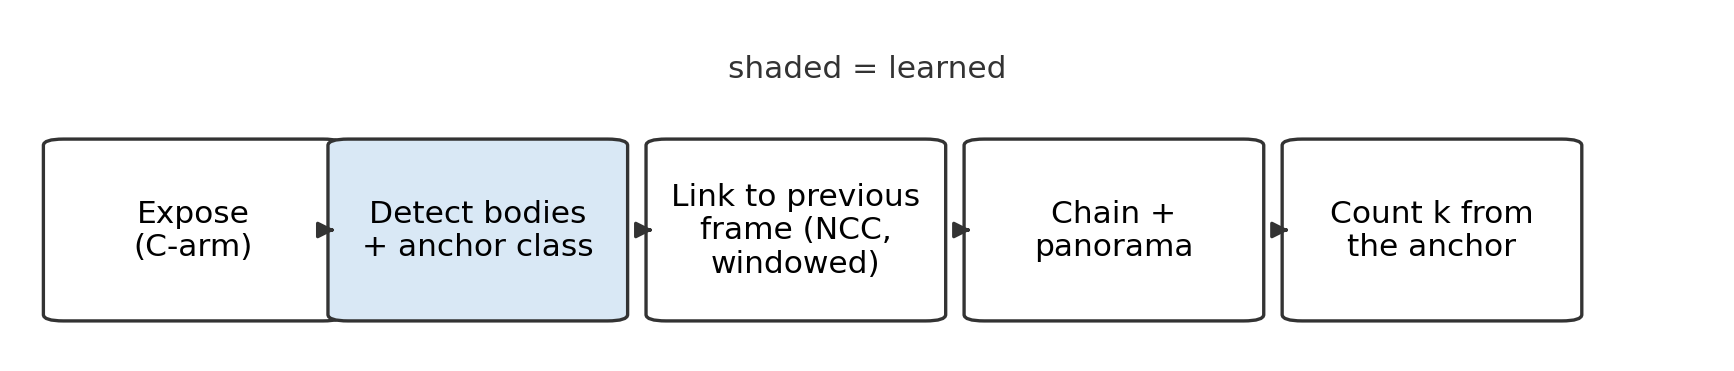
\includegraphics[width=\linewidth]{figures/fig1_pipeline.png}
\caption{The processing chain, end to end and without a branch. Only the shaded stage is learned. The
count consumes box positions and never reads a class, so no network takes part in the count.}
\label{fig:pipeline}
\end{figure}

\begin{figure}[htbp]\centering
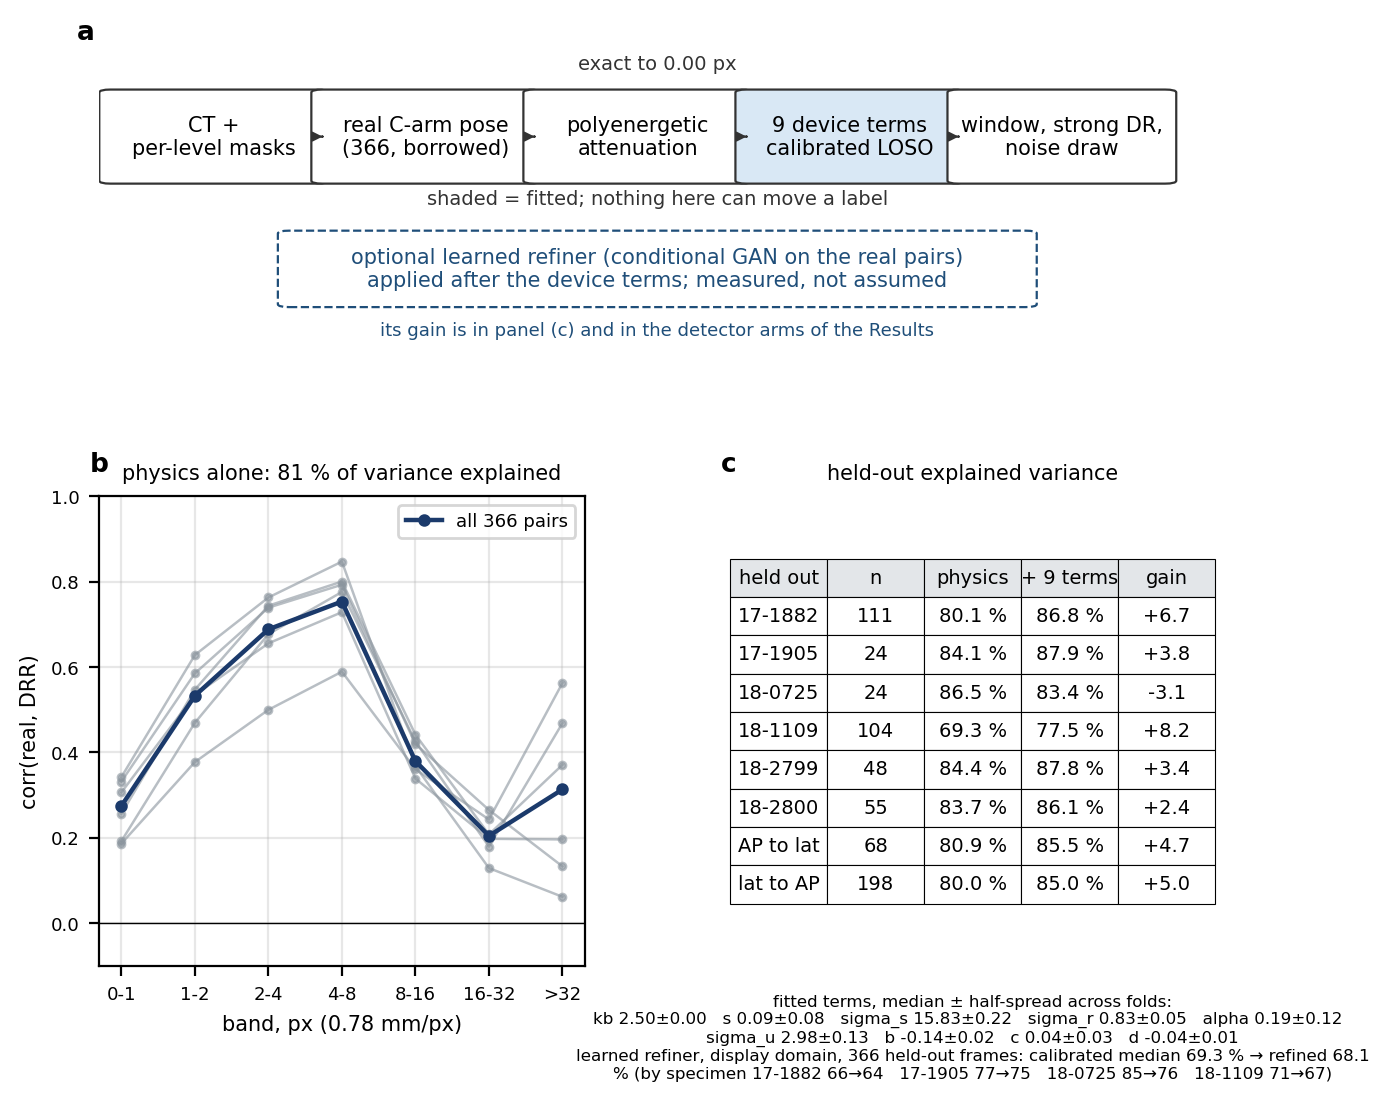
\includegraphics[width=\linewidth]{figures/fig_formation.png}
\caption{Image formation calibrated on real fluoroscopy. (a) Every stage; the shaded one is fitted, the dashed one the optional learned refiner, built and measured. (b) Agreement between the exact-geometry DRR and the real frame by band, all 366 pairs. (c) Held-out explained variance by specimen and by view angle, and the refiner's on the same frames.}
\label{fig:formation}
\end{figure}

\begin{figure}[p]
\centering
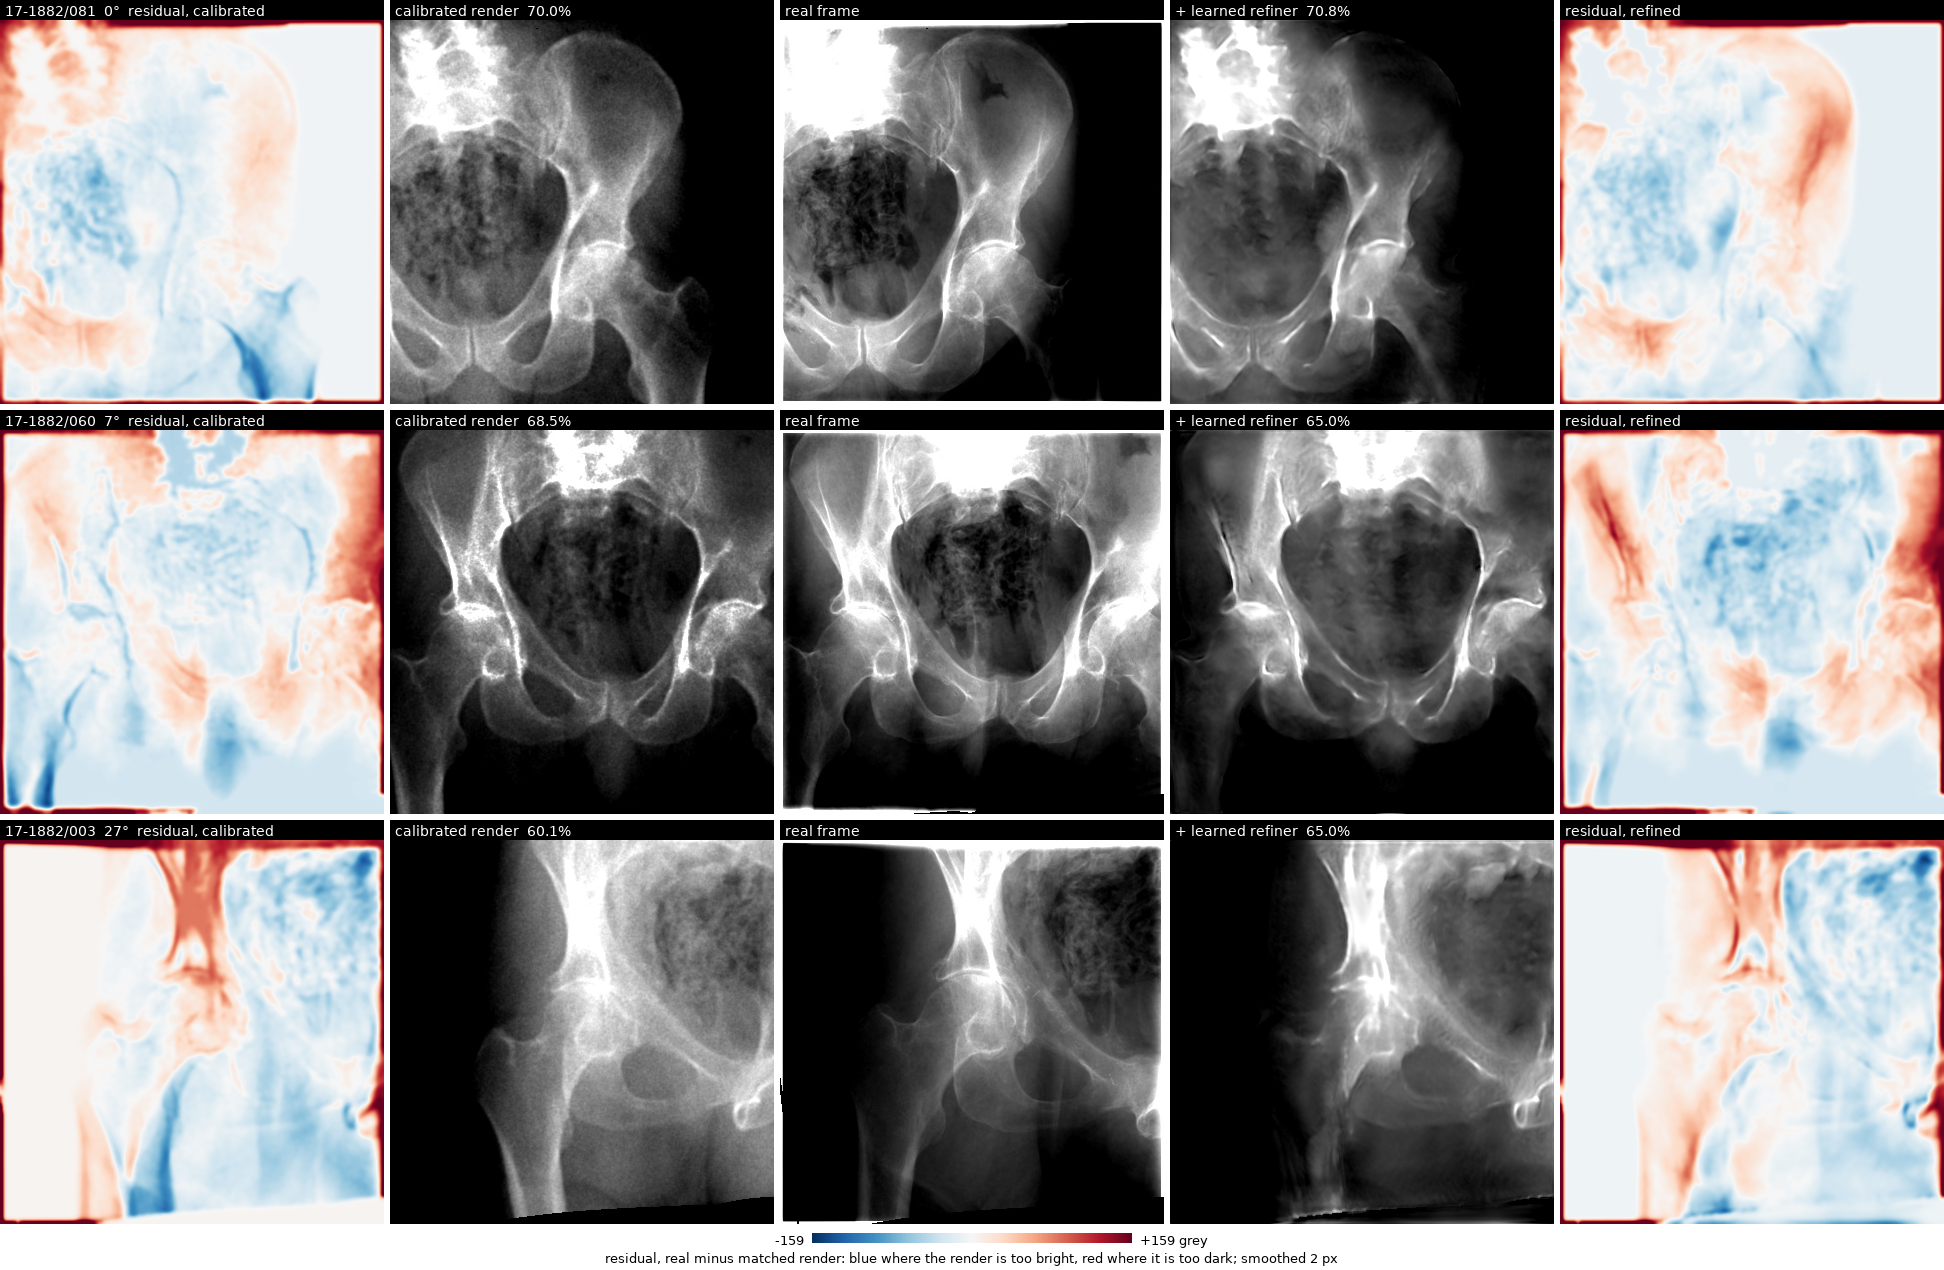
\includegraphics[width=\linewidth]{figures/fig_best_synthetic.png}
\caption{A held-out specimen at three lateral tilts. Centre, the real frame; left, the calibrated render of its own CT under the same pose, terms fitted with the specimen excluded; right, that render through the learned refiner. Outer columns, each render's signed residual: red where the render is too dark, blue too bright. Percentages, display variance explained.}
\label{fig:formation-spine}
\end{figure}

\begin{figure*}[t]
\centering
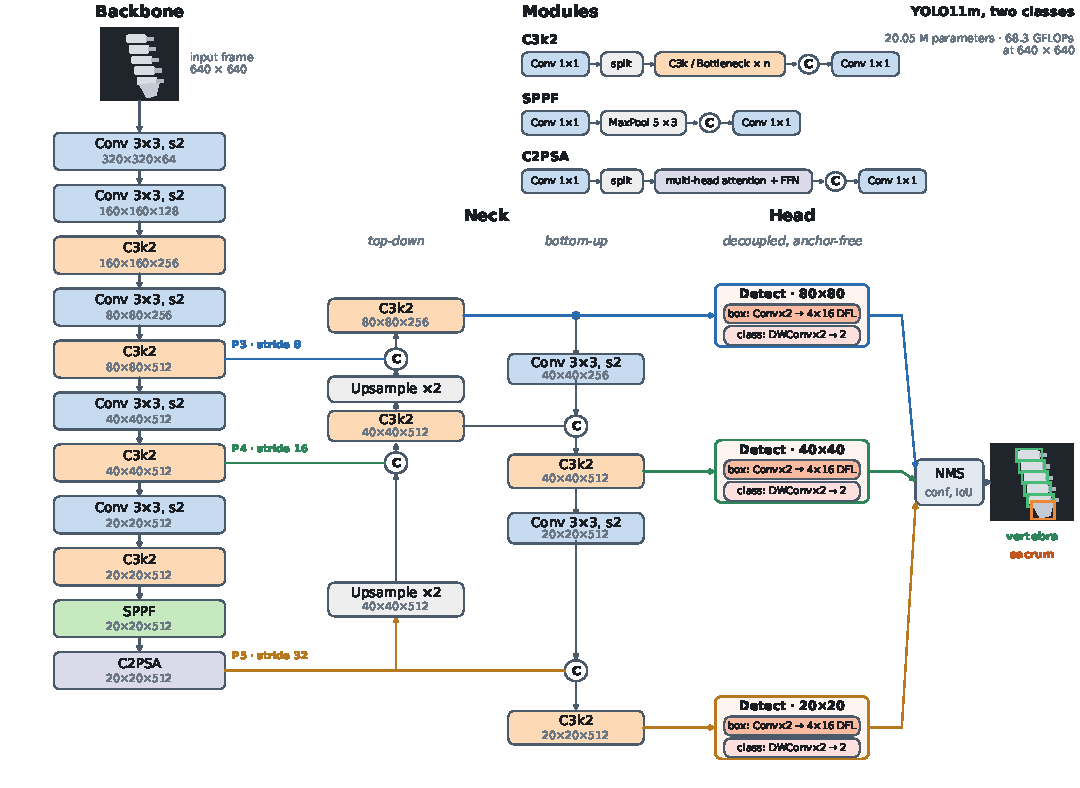
\includegraphics[width=\linewidth]{figures/fig_detector.pdf}
\caption{The two-class detector (YOLO11m; 20.05\,M parameters, 68.3 GFLOPs at 640\,$\times$\,640). A convolutional backbone with spatial pyramid pooling and position-sensitive attention feeds a top-down and bottom-up feature pyramid; decoupled anchor-free heads at strides 8, 16 and 32 predict box distributions and vertebra or sacrum scores, merged by non-maximum suppression.}
\label{fig:detector}
\end{figure*}

\begin{figure}[p]
\centering
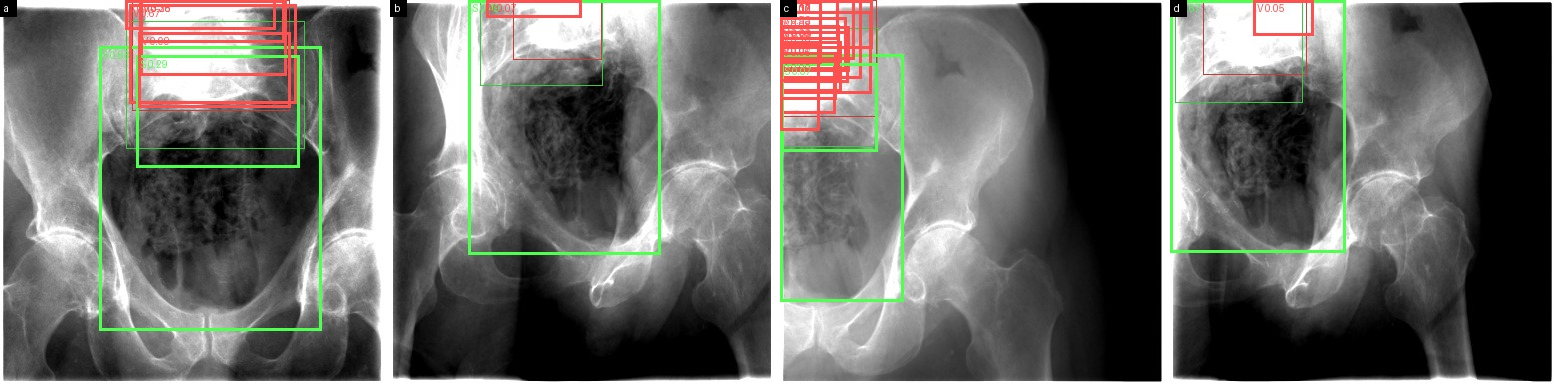
\includegraphics[width=\linewidth]{figures/fig_anchor_real.png}
\caption{A detector trained only on calibrated synthetic frames, on real fluoroscopy of a held-out
specimen. Thin boxes are the shipped segmentation (green sacrum, red vertebrae); thick boxes are calls at
confidence 0.05 with their scores. The sacrum is found in the upright frames; the saturated lumbosacral
region of an oblique frame collects low-confidence vertebra calls.}
\label{fig:anchor-real}
\end{figure}

\begin{figure}[htbp]\centering
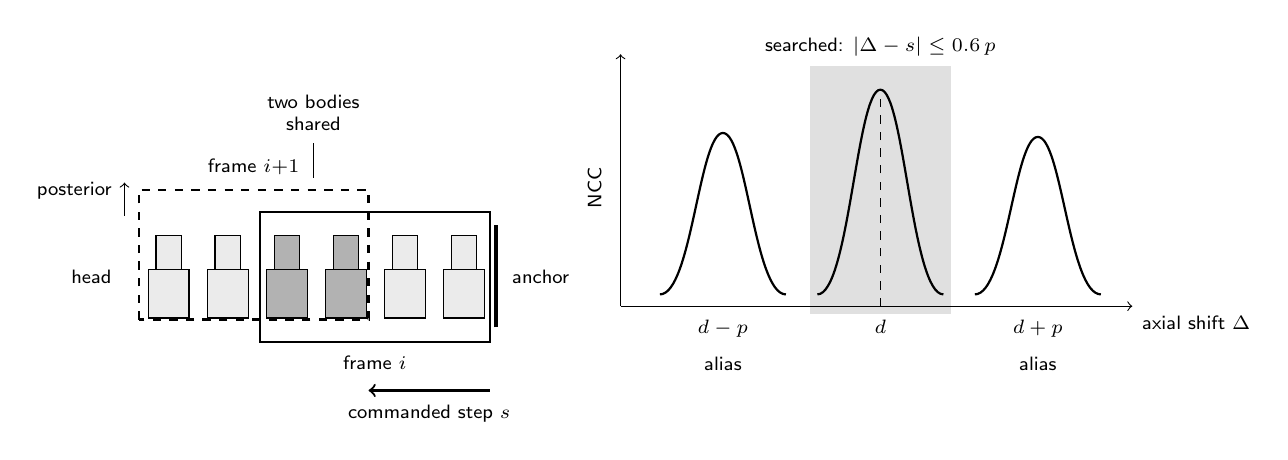
\begin{tikzpicture}[x=1cm,y=1cm]

% ---------------- left panel: two overlapping fields on one periodic column, PRONE.
% Head left, posterior up, sacral anchor at the right, so the sweep advances leftward and the schematic
% matches every x-ray panel in the paper. Each vertebra is a body with a posterior element on top.
\begin{scope}[shift={(0,0)}]
  \foreach \i in {0,...,5} {
    \draw[fill=black!8] (0.75*\i,0) rectangle (0.75*\i+0.52,0.62);
    \draw[fill=black!8] (0.75*\i+0.10,0.62) rectangle (0.75*\i+0.42,1.05);
  }
  \foreach \i in {2,3} {
    \draw[fill=black!30] (0.75*\i,0) rectangle (0.75*\i+0.52,0.62);
    \draw[fill=black!30] (0.75*\i+0.10,0.62) rectangle (0.75*\i+0.42,1.05);
  }
  \draw[very thick] (4.42,-0.12) -- (4.42,1.18);
  \node[font=\scriptsize,anchor=west] at (4.50,0.53) {anchor};

  \draw[thick] (1.42,-0.30) rectangle (4.34,1.35);
  \node[font=\scriptsize,anchor=north] at (2.88,-0.36) {frame $i$};

  \draw[thick,dashed] (-0.12,-0.02) rectangle (2.80,1.63);
  \node[font=\scriptsize,anchor=south] at (1.34,1.69) {frame $i{+}1$};

  \draw[<-,thick] (2.80,-0.92) -- (4.34,-0.92);
  \node[font=\scriptsize,anchor=north] at (3.57,-0.98) {commanded step $s$};

  \draw[-] (2.10,2.22) -- (2.10,1.78);
  \node[font=\scriptsize,anchor=south,align=center] at (2.10,2.26) {two bodies\\shared};

  % both orientation cues sit outside the frames; the arrow used to run through frame i+1
  \node[font=\scriptsize,anchor=east] at (-0.34,0.53) {head};
  \node[font=\scriptsize,anchor=east] at (-0.34,1.62) {posterior};
  \draw[->] (-0.30,1.30) -- (-0.30,1.72);
\end{scope}

% ---------------- right panel: correlation over axial shift
\begin{scope}[shift={(6.3,0.15)}]
  \fill[black!12] (2.1,-0.1) rectangle (3.9,3.05);
  \draw[->] (-0.3,0) -- (6.2,0) node[anchor=north west,font=\scriptsize] {axial shift $\Delta$};
  \draw[->] (-0.3,0) -- (-0.3,3.2);
  \node[font=\scriptsize,anchor=south,rotate=90] at (-0.42,1.5) {NCC};

  \draw[thick] (0.2,0.15) .. controls (0.6,0.15) and (0.7,2.2) .. (1.0,2.2)
                          .. controls (1.3,2.2) and (1.4,0.15) .. (1.8,0.15);
  \draw[thick] (2.2,0.15) .. controls (2.6,0.15) and (2.7,2.75) .. (3.0,2.75)
                          .. controls (3.3,2.75) and (3.4,0.15) .. (3.8,0.15);
  \draw[thick] (4.2,0.15) .. controls (4.6,0.15) and (4.7,2.15) .. (5.0,2.15)
                          .. controls (5.3,2.15) and (5.4,0.15) .. (5.8,0.15);

  \draw[dashed] (3.0,0) -- (3.0,2.75);
  \node[font=\scriptsize,anchor=north] at (1.0,-0.05) {$d-p$};
  \node[font=\scriptsize,anchor=north] at (3.0,-0.05) {$d$};
  \node[font=\scriptsize,anchor=north] at (5.0,-0.05) {$d+p$};
  \node[font=\scriptsize,anchor=south] at (3.0,3.05) {searched: $|\Delta-s|\le 0.6\,p$};
  \node[font=\scriptsize,anchor=north] at (1.0,-0.52) {alias};
  \node[font=\scriptsize,anchor=north] at (5.0,-0.52) {alias};
\end{scope}

\end{tikzpicture}
\caption{The C-arm's view of a prone patient: head left, posterior up. Left: consecutive fields share
two bodies after a commanded step $s$. Right: correlation over axial shift peaks at $d$ and again at
$d\pm p$, one body pitch away, because the column repeats. Searching within $0.6\,p$ of $s$ leaves the
aliases outside the search.}
\label{fig:mechanism}
\end{figure}

\begin{figure}[htbp]\centering
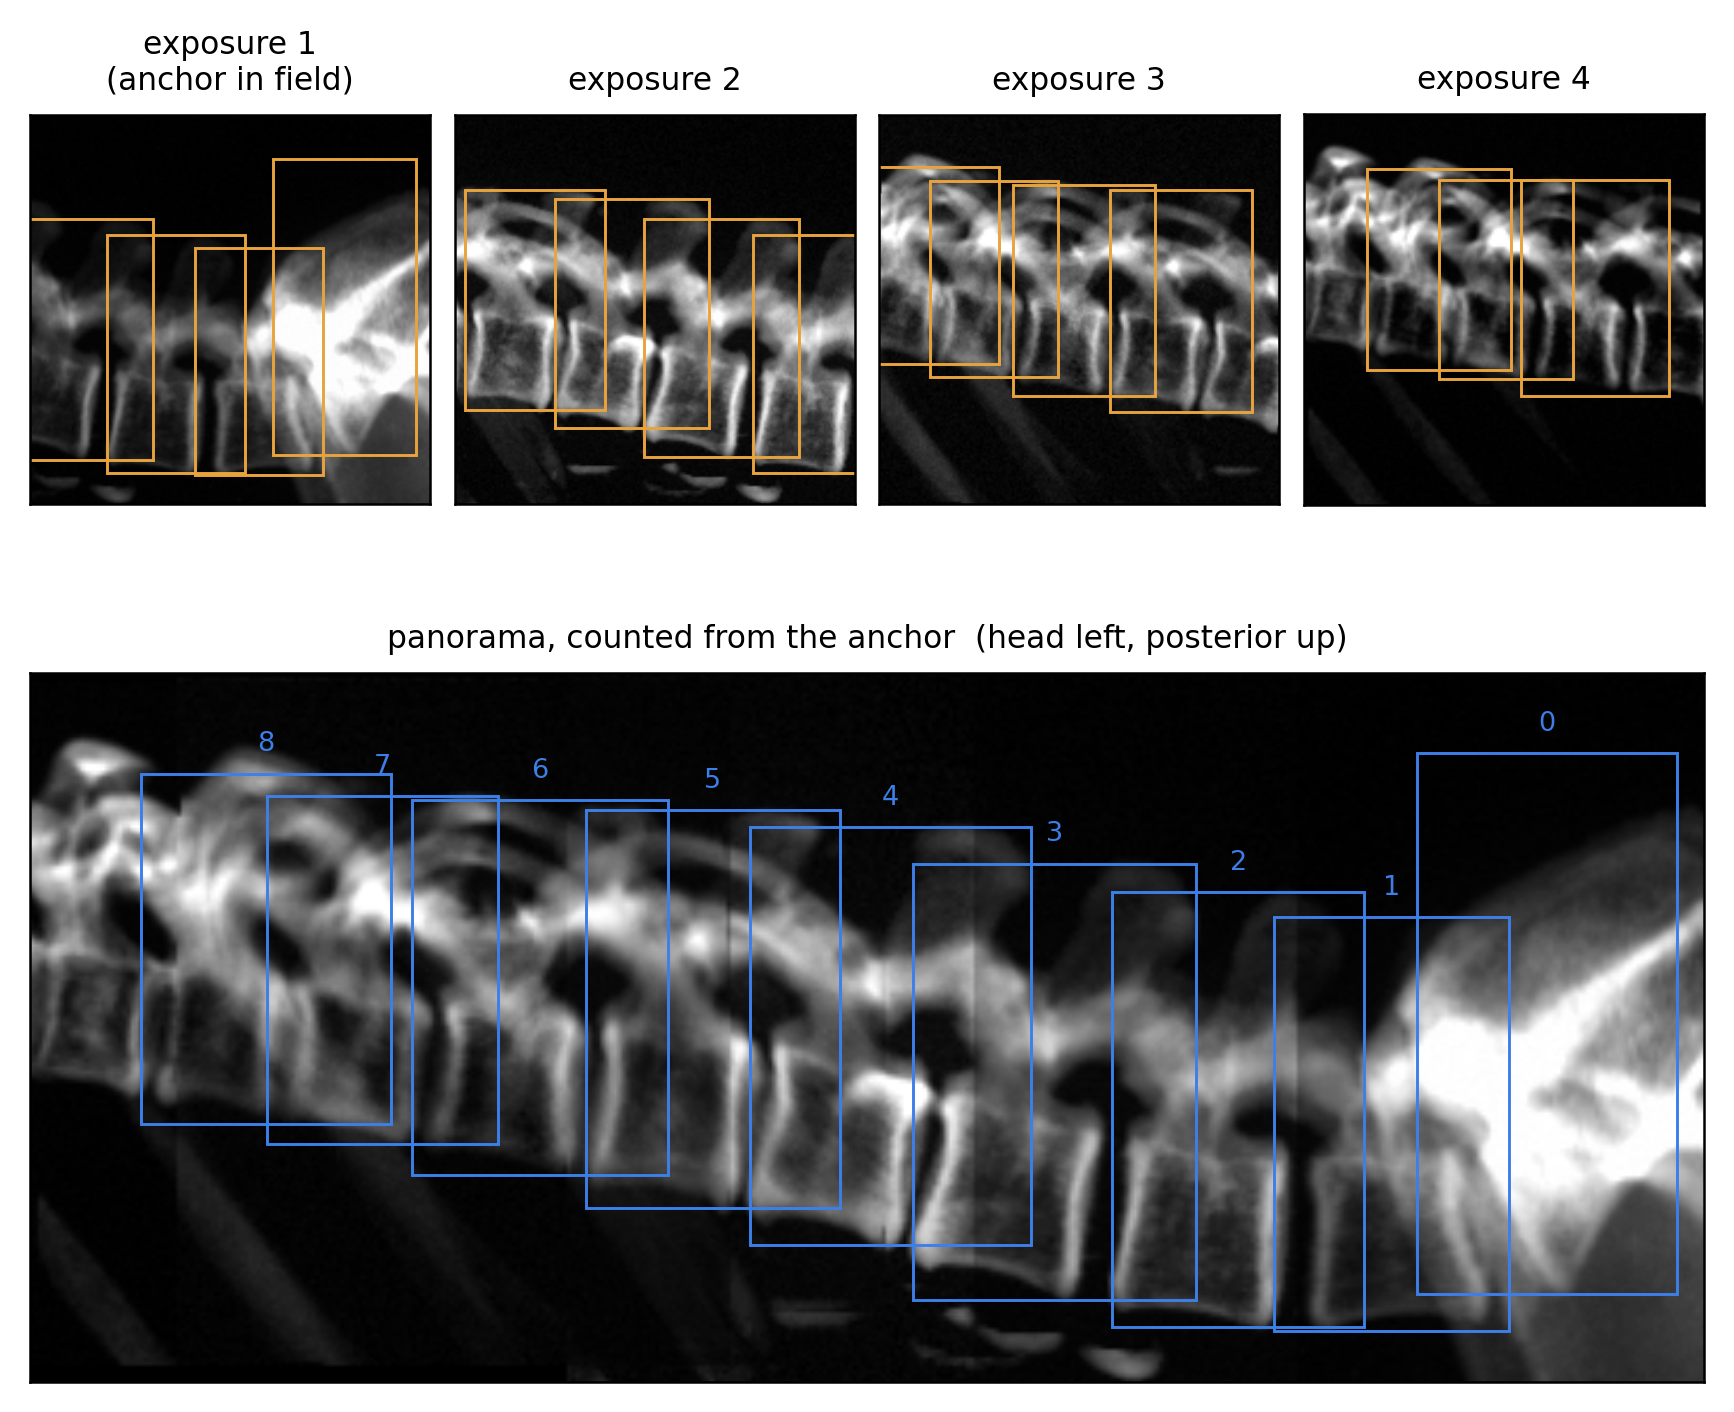
\includegraphics[width=\linewidth]{figures/fig2_stitch.png}
\caption{Four exposures of one spine and the chain they build, in the view a C-arm gives on a prone
patient: head left, posterior up, at true scale. Each field is degraded independently. Consecutive
frames are linked on their shared band and the nodes are numbered outward from the anchor. No node
carries a vertebra name.}
\label{fig:stitch}
\end{figure}

\begin{figure}[htbp]\centering
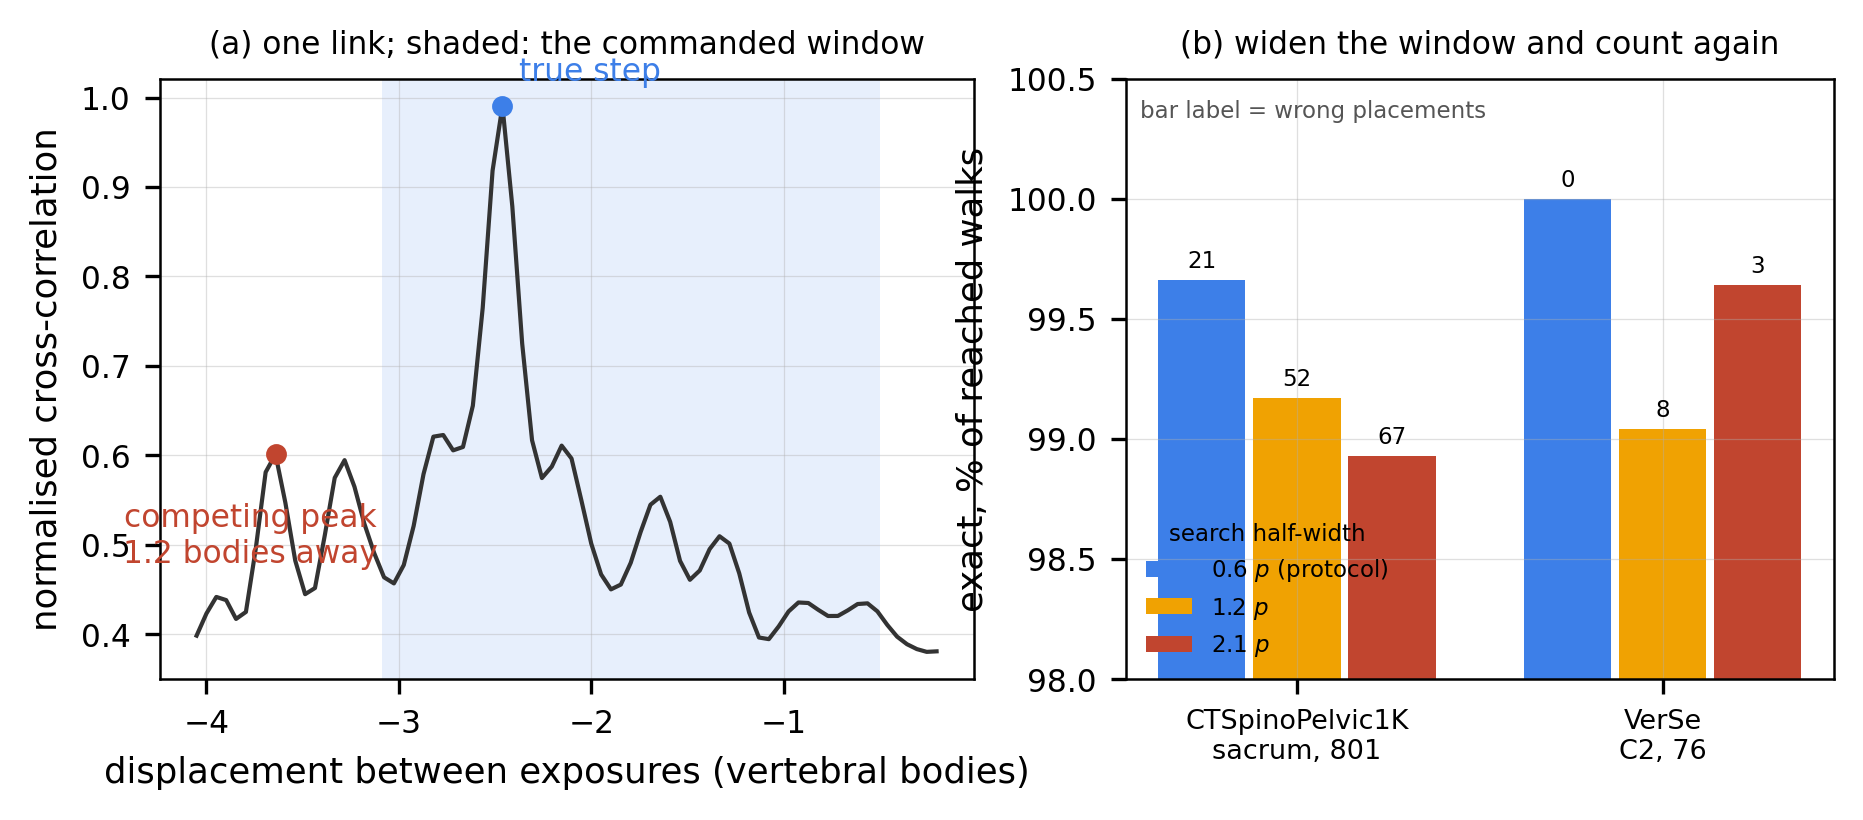
\includegraphics[width=\linewidth]{figures/fig3_step.png}
\caption{(a) Correlation over axial shift for one link; the true peak stands well above the competing
peak, so this link would survive an unconstrained search. (b) Widening the search on every spine: the
count survives a window 3.5 times too wide, so the restriction is not the mechanism. What it buys is the
last fraction.}
\label{fig:step}
\end{figure}

\begin{figure}[htbp]\centering
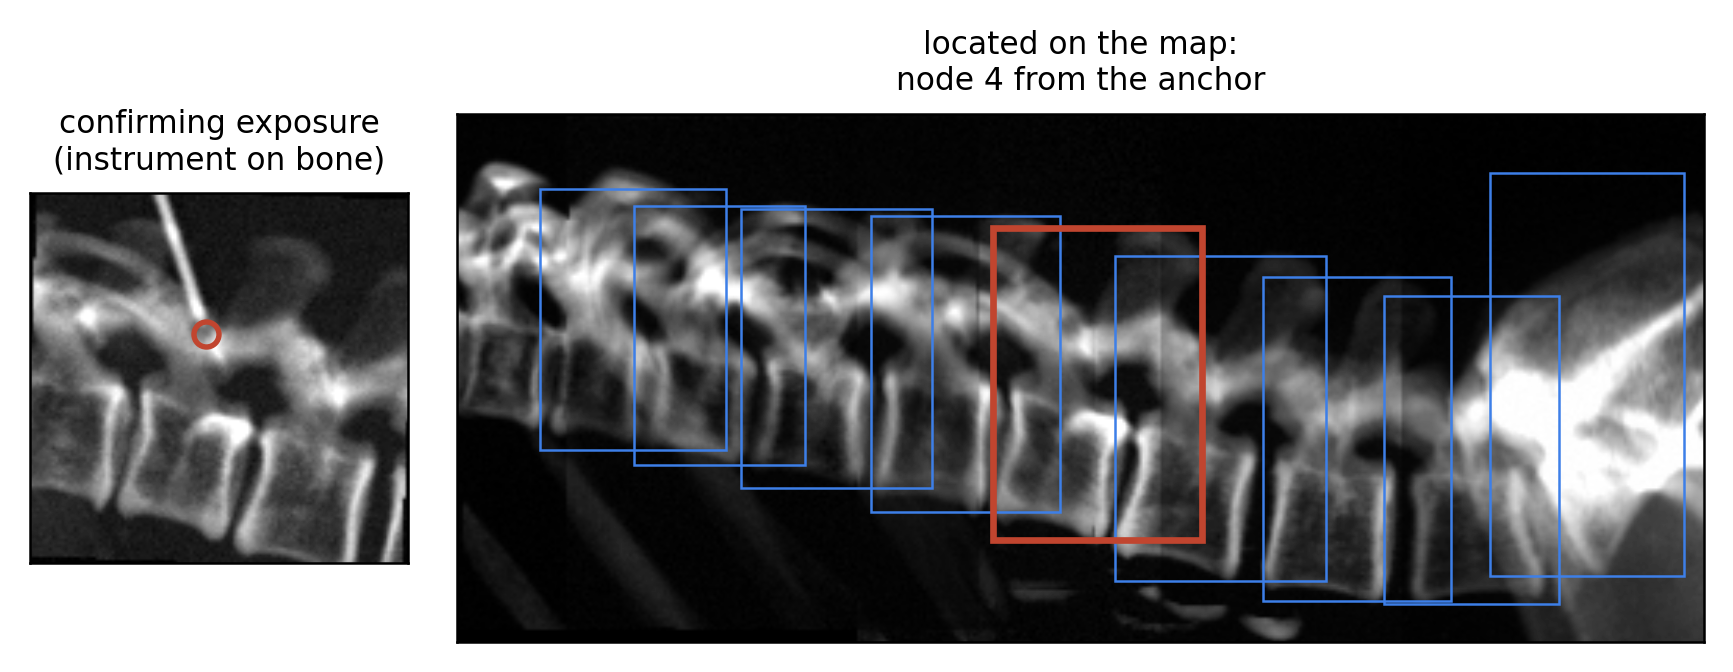
\includegraphics[width=0.86\linewidth]{figures/fig4_confirm.png}
\caption{Confirmation. An instrument enters from posterior and stops on the bone it touches; that one
exposure is matched onto the chain and the body under the tip carries its ordinal from the anchor. No
tracker and no preoperative CT. Panels are at true relative scale. The instrument is not free: see the
cervical result in the text.}
\label{fig:confirm}
\end{figure}

\begin{figure}[p]
\centering
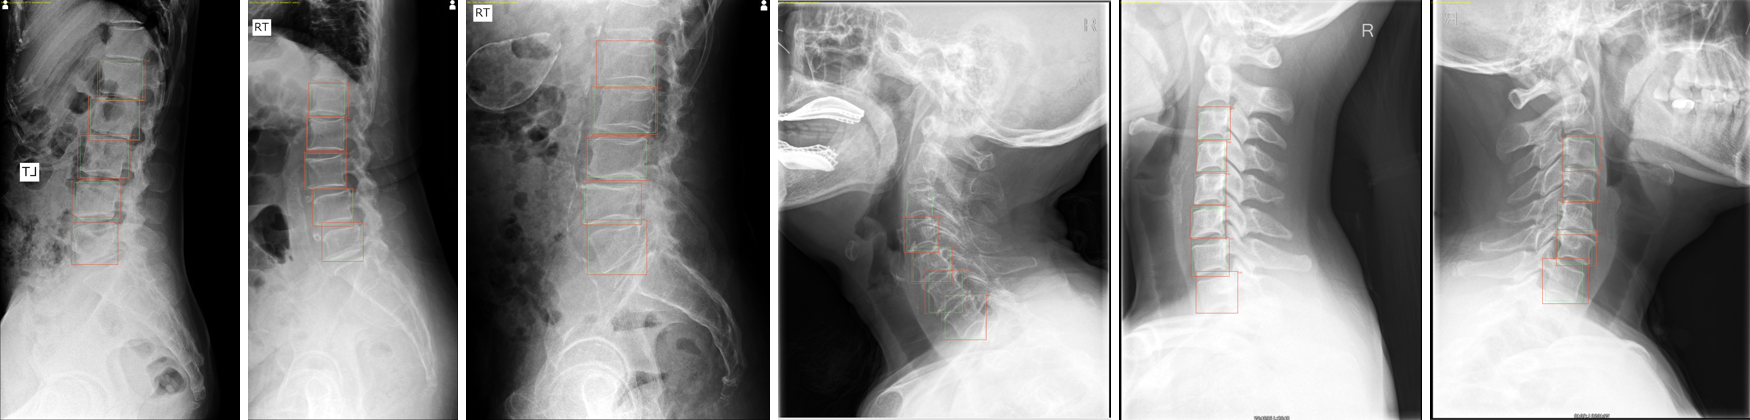
\includegraphics[width=\linewidth]{figures/fig_boxes_films.png}
\caption{The deployed film detector on real radiographs it was not trained on: three lumbar and three
cervical. Thin green boxes are the annotation; red boxes are the detector's calls at a confidence of
0.25 with their scores. One cervical film loses its lowest body; one carries an extra call.}
\label{fig:boxes-films}
\end{figure}

% ------------------------------------------------------------------------------------------------ TABLES
\clearpage

\begin{table}[htbp]\centering\footnotesize\setlength\tabcolsep{2.5pt}
\caption{The twelve counting arms run with the annotation's vertebra boxes. No learned component takes part,
so no spine is withheld. \emph{Reached} excludes walks whose target never entered a field; exactness is
scored on those, as a percentage with an exact binomial 95\,\% interval over walks, which ignores
clustering within spines. \emph{Wrong} gives wrong walks with distinct spines in parentheses. Refusals were
zero in every row and the anchor diagnostic was 100\,\% except in the 522-spine sacrum arm (99.35\,\%). The
C2 arms on the second institution also carry 43 sacral targets, not broken out above: 42 of 43 were exact
at two bodies of overlap, and at three every one of the 41 that reached was exact, two never reaching. CTSP1K is CTSpinoPelvic1K; TotalSeg.\ is TotalSegmentator's public release; C, T and L
are exactness on cervical, thoracic and lumbar targets.}
\label{tab:count}
\begin{tabular}{llrrrlrrrrr}
\toprule
Anchor, ovl. & Corpus & Spines & Walks & Reach. & Exact \%\ (95\,\% CI) & C & T & L & Exp. & Wrong \\
\midrule
C2, 2   & VerSe        &  76 &   834 &   834 & 99.76 (99.14--99.97) & 100 & 99.46 & 100 & 1.99 &  2 (1) \\
C2, 3   & VerSe        &  76 &   834 &   834 & 100 (99.56--100)     & 100 & 100   & 100 & 2.24 &  0 (0) \\
C2, 2   & TotalSeg.    & 204 & 2{,}656 & 2{,}654 & 99.70 (99.41--99.87) & 100 & 99.71 & 97.87 & 2.05 &  8 (2) \\
C2, 3   & TotalSeg.    & 204 & 2{,}656 & 2{,}650 & 99.62 (99.31--99.82) & 100 & 99.41 & 97.45 & 2.27 & 10 (2) \\
C2, 2   & Radiographs & 262 & 1{,}209 & 1{,}209 & 99.67 (99.16--99.91) & 99.66 & 100 & --- & 1.13 &  4 (4) \\
C2, 3   & Radiographs & 264 & 1{,}217 & 1{,}217 & 99.42 (98.82--99.77) & 99.50 & 96.30 & --- & 1.13 &  7 (3) \\
C2, 2   & Radiographs$^{*}$ &  24 &   110 &   110 & 100 (96.70--100)     & 100 & 100 & --- & 1.15 &  0 (0) \\
C2, 3   & Radiographs$^{*}$ &  24 &   110 &   110 & 100 (96.70--100)     & 100 & 100 & --- & 1.15 &  0 (0) \\
\midrule
Sac., 2 & CTSP1K & 801 & 6{,}352 & 6{,}255 & 99.66 (99.49--99.79) & --- & 95.45 & 99.73 & 1.98 & 21 (6) \\
Sac., 3 & CTSP1K & 801 & 6{,}352 & 6{,}229 & 99.76 (99.60--99.87) & --- & 94.51 & 99.78 & 2.42 & 15 (5) \\
Sac., 2 & TotalSeg.    & 522 & 7{,}396 & 7{,}228 & 99.17 (98.93--99.37) & 83.84 & 97.41 & 99.33 & 2.96 & 60 (6) \\
Sac., 2 & Radiographs$^{*}$ &  16 &    95 &    95 & 100 (96.19--100)     & --- & 100 & 100 & 1.61 &  0 (0) \\
\bottomrule
\end{tabular}

\vspace{2pt}
\raggedright\scriptsize $^{*}$Films held out from the film detector. The 262-film arm uses every annotated
lateral radiograph that carries C2, because counting fits nothing.
\end{table}

\begin{table}[htbp]\centering\footnotesize\setlength\tabcolsep{4pt}
\caption{Where the residual risk is. The first five rows are the same 79 abdominopelvic spines, held out
from the render-trained detector and counted from the sacrum under five box and anchor conditions; the
first is this table's true-box control. The last three are real lateral radiographs held out from the film
detector. \emph{Anchor} is the share of walks whose starting node really was the anchor. Exactness carries
an exact binomial 95\,\% interval over walks, which ignores clustering within spines.}
\label{tab:boxes}
\begin{tabular}{lllrrrlrrr}
\toprule
Boxes, anchor rule & Anchor & Ovl. & Spines & Walks & Reach. & Exact (95\,\% CI) & Anchor & Wrong & Ref. \\
\midrule
Annotation, terminal      & Sacrum & 2 & 79 & 625 & 618 & 100 (99.40--100)     & 100   &   0 (0) &   0 \\
Render detector, terminal & Sacrum & 2 & 79 & 625 & 622 & 30.06 (26.48--33.84) & 42.44 & 435 (79) &   0 \\
Render detector, terminal & Sacrum & 3 & 79 & 625 & 621 & 28.66 (25.14--32.40) & 39.77 & 443 (75) &   0 \\
Render detector, class    & Sacrum & 2 & 79 & 625 & 118 & 44.07 (34.94--53.50) & 100   &  66 (15) & 507 \\
Render detector, class    & Sacrum & 3 & 79 & 625 &  96 & 43.75 (33.64--54.25) & 100   &  54 (11) & 529 \\
\midrule
Film detector, terminal   & Sacrum & 2 & 16 &  95 &  95 & 100 (96.19--100)     & 93.68 &   0 (0) &   0 \\
Film detector, class      & Sacrum & 2 & 16 &  95 &   0 & ---                  & ---   &   0 (0) &  95 \\
Film detector, terminal   & C2     & 2 & 24 & 110 & 107 & 29.91 (21.44--39.52) & 93.46 &  75 (21) &   0 \\
\bottomrule
\end{tabular}
\end{table}

\clearpage
\bibliographystyle{unsrtnat}
\bibliography{../rsnai/refs}

\end{document}

% =====================================================================================================
% REVIEWER NOTES -- fixes considered and the reason each was not applied as written.
%
% 1. "Report the C2 real-film arm as 1,204 of 1,209 (99.67 %)." NOT APPLIED as written: 1,204/1,209 is
%    99.59 %, not 99.67 %. The generated table gives reached 1,209, exact 0.9967 and wrong 4, so the
%    numerator is 1,205. The narrative paragraph of docs/COUNTING_EVIDENCE.md disagrees with its own
%    table by one and should be regenerated. 1,205 is used here.
%
% 2. "Add Clopper-Pearson intervals to EVERY proportion, including the abstract." Applied to every
%    proportion whose numerator is an integer recoverable from the generated tables (reached minus
%    wrong). NOT applied to the naming arms (0.9625 of 950 walks, 0.9469 of 7,405) or to the needle
%    arms, because the evidence files give those as rounded proportions over a denominator that is not
%    the printed walk count, so no exact numerator can be recovered without regenerating the briefs.
%    Inventing one to obtain an interval is the failure mode this paper is written against.
%
% 3. "Name the film corpus, its total size and its selection." Applied for the collections and the arm
%    sizes. NOT applied for the corpus total (9,109 films): that figure lives in
%    docs/MANIFEST_DATA_MODELS_RESULTS.md, which is not one of the five evidence briefs the header
%    declares as this paper's only numeric source.
%
% 4. "Rename the desilva2016 key, whose entry is authored by Lo et al." NOT APPLIED: refs.bib is shared
%    with paper/rsnai and the willingness-to-wait figure is attributed in SWEEP_TIME_EVIDENCE.md to
%    De Silva 2016, PMC5045321, PMID 27035579 -- the same PMID the Lo entry carries in its note. Which
%    author list belongs to that PMID has to be settled against the article itself, not guessed here.
%    The n = 3 the fix asked for has been added to the sentence.
%
% 5. "Rename mayer2008 to mayer2014." NOT APPLIED for the same reason: the key is shared with
%    paper/rsnai, where it resolves correctly to the 2014 Spine J article. The region and the
%    multiple-response design the fix asked for have been added to the sentence.
%
% 6. "Say the 6.25 duplicates per spine is unverified, or cite its result file." Deleted outright; no
%    result file in the tree carries a duplication rate, so the text now says the rate was not
%    quantified.
%
% 7. "Give the exposure count by distance from the anchor." Applied as the protocol's own figures
%    (three or four lumbar, six or seven mid-thoracic). A per-target-distance distribution of exposures
%    is not in any evidence file and is not reported.

% 8. Length. The brief set 2,800--3,400 words of main text. The manuscript stands at 4,030 with
%    Introduction through Conclusion, counted with LaTeX markup and citations stripped, and the earlier
%    draft stood at about 3,400. The overrun is the fixes: the C2 real-film arm, the per-region
%    breakdowns for every corpus, the needle-confirmation subsection and its control, the third
%    detector-box condition, the third class-anchor arm, the jitter arm, the confidence intervals, the
%    survey denominators and response rates, and the disclaimers on navigation, registration, reader
%    performance and site of care. Meeting 3,400 now requires dropping one of those, and each was a
%    blocker. If a cut is required, the candidates in order are the cost-to-run subsection (about 165
%    words, duplicated in part by the Discussion), the burden extrapolation in the Introduction (about
%    90) and the spot-image naming figures, which Table 1 and the walk-level arms do not need.
% =====================================================================================================
